%========== Preamble ==========
\documentclass[a4paper,12pt]{article}

% NOTE: the bidi package (loaded internally by polyglossia) requires that
% caption, hyperref, xcolor, geometry, titlesec, etc. all be loaded BEFORE
% polyglossia. fontspec + polyglossia + language setup therefore comes last.
% The `article` class is used (rather than KOMA's scrartcl) because bidi
% ships dedicated, well-tested patches for the standard LaTeX classes.

% ---------- Math ----------
\usepackage{amsmath,amsfonts,amssymb}

% ---------- Page geometry ----------
\usepackage[left=2.6cm, right=2.6cm, top=2.8cm, bottom=2.8cm, headsep=1.1cm]{geometry}

% ---------- Colors ----------
\usepackage{xcolor}
\definecolor{ruppinblue}{RGB}{40,76,117}
\definecolor{ruppingreen}{RGB}{119,186,81}
\definecolor{ruppingray}{RGB}{90,90,90}
\definecolor{lightgray}{RGB}{245,245,245}

% ---------- Graphics / floats ----------
\usepackage{graphicx}
\usepackage{float}

% ---------- Tables ----------
\usepackage{tabularx}
\usepackage{booktabs}
\usepackage{multirow}
\usepackage{array}
\newcolumntype{L}[1]{>{\RaggedRight\arraybackslash}p{#1}}
\newcolumntype{C}[1]{>{\Centering\arraybackslash}p{#1}}

% ---------- Captions ----------
\usepackage{caption}
\captionsetup{
  format=plain,
  labelfont={bf,color=ruppinblue},
  font=small,
  justification=centerlast,
  singlelinecheck=false,
  skip=6pt
}

% ---------- Lists ----------
% NOTE: LaTeX's standard `list` environment (which itemize/enumerate/enumitem
% all build on) mis-places its label for single-line items under bidi/RTL --
% the label ends up anchored to the LTR-assumed side, so a short one-line
% item's bullet/number visibly shifts left relative to multi-line items in
% the same list, even though multi-line items wrap correctly. Plain
% \hangindent-based paragraphs do not have this bug, so itemize/enumerate are
% redefined below to use \hangindent directly instead of LaTeX's `list`
% machinery. This is a document-wide override: every \begin{itemize}/
% \begin{enumerate} in the section files uses this automatically.
\usepackage{enumitem} % kept loaded but itemize/enumerate below bypass it
\makeatletter
\renewenvironment{itemize}
  {\par\begingroup
   \def\item{\par\noindent\hangindent=1.45em\hangafter=1
     \makebox[1.45em][r]{\textbullet\hspace{0.55em}}\ignorespaces}}
  {\par\endgroup}

\newcounter{hebenumctr}
\renewenvironment{enumerate}
  {\par\begingroup\setcounter{hebenumctr}{0}%
   \def\item{\par\noindent\stepcounter{hebenumctr}\hangindent=1.45em\hangafter=1
     \makebox[1.45em][r]{\thehebenumctr.\hspace{0.4em}}\ignorespaces}}
  {\par\endgroup}
\makeatother

% ---------- Section heading styling ----------
\usepackage{titlesec}
\titleformat{\section}
  {\color{ruppinblue}\Large\bfseries}{\thesection.}{0.5em}{}
  [{\color{ruppingreen}\titlerule[1pt]}]
\titleformat{\subsection}
  {\color{ruppinblue}\large\bfseries}{\thesubsection}{0.5em}{}
\titleformat{\subsubsection}
  {\color{ruppinblue!85!black}\normalsize\bfseries}{\thesubsubsection}{0.5em}{}
\titlespacing*{\section}{0pt}{1.6\baselineskip}{0.9\baselineskip}
\titlespacing*{\subsection}{0pt}{1.1\baselineskip}{0.6\baselineskip}
\titlespacing*{\subsubsection}{0pt}{0.9\baselineskip}{0.4\baselineskip}

% ---------- Header / Footer ----------
\usepackage{fancyhdr}
\pagestyle{fancy}
\fancyhf{}
\renewcommand{\headrulewidth}{0pt}
\fancyhead[C]{\small\color{ruppingray}פיתוח מודל למידת מכונה לחיזוי משתני בית שורשים בחממה}
\fancyfoot[C]{\small\color{ruppingray}\thepage}
\fancypagestyle{plain}{%
  \fancyhf{}
  \fancyfoot[C]{\small\color{ruppingray}\thepage}
  \renewcommand{\headrulewidth}{0pt}
}

% ---------- Misc ----------
\usepackage{setspace}
\onehalfspacing
\setlength{\parindent}{0pt}
\setlength{\parskip}{0.55em}
\clubpenalty=10000
\widowpenalty=10000
\setcounter{secnumdepth}{3}
\setcounter{tocdepth}{2}

% ---------- Hyperlinks ----------
\usepackage[
  pdftitle={פיתוח מודל למידת מכונה לחיזוי משתני בית שורשים בחממה},
  pdfauthor={עדן אליהו, אורן צ'אושו},
  colorlinks=true,
  linkcolor=ruppinblue,
  urlcolor=ruppinblue,
  citecolor=ruppinblue,
  breaklinks=true
]{hyperref}

% ---------- Fonts & language (XeLaTeX + Hebrew RTL) ----------
\usepackage{fontspec}
\usepackage{polyglossia}
\setmainlanguage{hebrew}
\setotherlanguage{english}

\setmainfont{David}
\newfontfamily\hebrewfont[Script=Hebrew]{David}
\newfontfamily\englishfont{Times New Roman}

% Non-breaking LTR terms inside Hebrew paragraphs. These prevent English
% technical terms from splitting across lines and starting visually misaligned.
\newcommand{\ltrterm}[1]{\textenglish{#1}}
\newcommand{\GB}{\textenglish{Gradient~Boosting}}
\newcommand{\WFV}{\textenglish{Walk-Forward~Validation}}
\newcommand{\SoftSensor}{\textenglish{Soft~Sensor}}
\newcommand{\Rtwo}{\textenglish{$R^2$}}

% Figure/Table labels stay in Hebrew ("איור"/"טבלה", set automatically by
% polyglossia's Hebrew module); caption descriptions themselves stay in
% English via explicit \LR{} wrapping at each \caption call.

% ---------- Document info ----------
\newcommand{\projtitle}{פיתוח מודל למידת מכונה לחיזוי משתני בית שורשים בחממה}
\newcommand{\projnum}{14}
\newcommand{\authorone}{עדן אליהו}
\newcommand{\authortwo}{אורן צ'אושו}
\newcommand{\supervisorone}{ד"ר אבנר פריאל}
\newcommand{\supervisortwo}{ד"ר עלאא ג'מאל}

%========== Begin of the document ==========
\begin{document}

\thispagestyle{empty}
\newgeometry{left=1.8cm, right=1.8cm, top=2.8cm, bottom=2.8cm}
\enlargethispage{2cm}
\begin{center}


\includegraphics[width=17cm]{figures/ruppin_logo.png}

\vspace{0.7cm}
{\LARGE\bfseries המחלקה למדעי המחשב} \\
{\Large הפקולטה להנדסה}

\vspace{1.1cm}
{\color{ruppingreen}\rule{\textwidth}{1.4pt}}

\vspace{0.7cm}
{\Large דוח מסכם פרויקט} \\[0.15cm]
{\Large מוגש כחלק מהדרישות לקבלת התואר "בוגר במדעים" \LR{(B.Sc.)} במדעי המחשב}

\vspace{1.2cm}
{\color{ruppinblue}\huge\bfseries פרויקט מספר \projnum} \\[0.35cm]
{\Huge\bfseries \projtitle}

\vspace{1.2cm}
{\color{ruppingreen}\rule{\textwidth}{1.4pt}}
\vspace{1.3cm}

\begin{tabular}{c}
\Large מוגש על-ידי: \\[0.3cm]
{\LARGE\bfseries \authorone} \\[0.15cm]
{\LARGE\bfseries \authortwo}
\end{tabular}

\vspace{1.3cm}

\begin{tabular}{c}
\Large בהנחיית: \\[0.3cm]
{\LARGE\bfseries \supervisorone} \\[0.15cm]
{\LARGE\bfseries \supervisortwo}
\end{tabular}

\vfill
{\Large המרכז האקדמי רופין}

\end{center}
\restoregeometry


\newpage
\pagenumbering{Roman}
\tableofcontents

\newpage
\renewcommand{\listfigurename}{רשימת איורים}
\section*{\listfigurename}
\begin{LTR}
\noindent\begin{tabularx}{\textwidth}{@{}r@{\quad}>{\raggedright\arraybackslash}X@{\quad}r@{}}
4  & Current Workflow -- Manual Sampling with Late Detection and Reactive Correction & 1 \\
5  & Physical-Biological Basis of Rootzone Dynamics & 2 \\
12 & Literature Review -- Comparative Analysis of Related Methods & 3 \\
14 & Historical Microclimate Data Imputation Results & 4 \\
15 & System Architecture -- Two-Stage Prediction Architecture & 5 \\
16 & Data Integration Pipeline -- Unified Master Dataset Construction & 6 \\
17 & Walk-Forward Validation Strategy & 7 \\
19 & Microclimate Model Results -- Parity Plot & 8 \\
20 & Rootzone Model Results -- Scatter Plot & 9 \\
21 & Rootzone Model Results -- Time-Series Prediction & 10 \\
22 & Baseline Comparison -- Model vs.\ Naive Predictors & 11 \\
26 & Digital Interface -- Weather Upload and Climate Forecast & 12 \\
26 & Digital Interface -- Operational Inputs & 13 \\
27 & Digital Interface -- Rootzone pH and EC Forecast & 14
\end{tabularx}
\end{LTR}
\addcontentsline{toc}{section}{רשימת איורים}

\renewcommand{\listtablename}{רשימת טבלאות}
\section*{\listtablename}
\begin{LTR}
\noindent\begin{tabularx}{\textwidth}{@{}r@{\quad}>{\raggedright\arraybackslash}X@{\quad}r@{}}
18 & Overall Micro-Climate Model Performance & 1 \\
21 & Rootzone Model Performance: Walk-Forward and Holdout & 2
\end{tabularx}
\end{LTR}
\addcontentsline{toc}{section}{רשימת טבלאות}

\newpage
\pagenumbering{arabic}
\setcounter{page}{1}

\section{תקציר}

\subsection{מטרת העבודה}
מטרת פרויקט זה היא לפתח מודל חיזוי דינמי מבוסס למידת מכונה \LR{(Machine Learning)} לניהול ולניטור משתני בית השורשים בחממה.

הפרויקט מתמקד ביצירת מערכת חיזוי מסוג \SoftSensor{} המסוגלת לחזות את ערכי המוליכות החשמלית (EC) והחומציות (pH) העתידיים בין מדידות ידניות דלילות, בהינתן נקודת מוצא ידועה (מדידה נוכחית).

המודל משקלל שלושה וקטורים עיקריים כדי לבצע את החיזוי:

\begin{itemize}
    \item \textbf{מצב התחלתי:} ערכי ה-EC וה-pH שנמדדו בנקודת הזמן הנוכחית.
    \item \textbf{תנאי סביבה:} נתוני אקלים חיצוני ומיקרו־אקלים בתוך החממה, לרבות קרינה, טמפרטורה, לחות, התאדות וטמפרטורת קרקע.
    \item \textbf{ממשק גידול:} נתוני השקיה, דישון, חומצה, מלחים ומועדי אירועים תפעוליים, לצד משתני מצב הצמח כגון כיסוי נוף וגיל הצמח.
\end{itemize}

\subsection{הערך היישומי}
יכולת חיזוי זו נועדה לשמש ככלי תומך החלטה עבור המגדל. היא מאפשרת לעבור מגישה תגובתית, שבה מתקנים חריגות לאחר שהתרחשו, לגישה פרואקטיבית, שבה ניתן לזהות מראש מגמות של שינויי מליחות או חומציות ולהתאים את משטר ההשקיה והדישון בהתאם.

באופן זה, המודל עשוי לסייע בשמירה על תנאים יציבים יותר בבית השורשים, בצמצום שימוש עודף במים ובדשן, ובהפחתת הסיכון לפגיעה בהתפתחות הצמח. עם זאת, בשלב הנוכחי המודל מיועד ככלי תומך החלטה ואינו מהווה מערכת בקרה אוטונומית.

\subsection{שיטת המחקר}
המחקר מתבסס על אינטגרציה של נתונים ממספר מקורות מידע, היוצרים יחד תמונת מצב רחבה של סביבת הגידול ושל פעולות הממשק בחממה:

\begin{itemize}
    \item \textbf{נתוני אקלים חיצוני:} נתוני קרינה, טמפרטורה, לחות ומשתני מזג אוויר נוספים.
    \item \textbf{נתוני חיישנים בחממה:} מדידות מיקרו-אקלים, לרבות טמפרטורה, לחות, התאדות ונתוני טמפרטורת קרקע.
    \item \textbf{נתוני תכנון גידול:} אירועי השקיה, דישון, שימוש בחומצה ומלחים, כמויות ומועדי יישום.
    \item \textbf{נתוני התפתחות הצמח:} כיסוי נוף וגיל הצמח, המשמשים לייצוג מצב הגידול וצריכת המים.
    \item \textbf{מדידות בית שורשים:} מדידות ידניות של pH ו-EC המשמשות כערכי יעד לאימון ולבדיקת המודל.
\end{itemize}

בסיס הנתונים הסופי נבנה כציר זמן אחיד ברזולוציה של 10 דקות וכלל 16{,}682 רשומות בטווח התאריכים 29.05.2025 עד 21.09.2025. עם זאת, מדידות היעד של pH ו-EC היו דלילות יחסית וכללו 109 נקודות מדידה בלבד. לכן, אחד האתגרים המרכזיים בפרויקט היה פיתוח מודל המסוגל ללמוד מתוך שילוב בין נתוני חיישנים צפופים לבין מדידות יעד ידניות ודלילות.

על בסיס נתונים אלו פותחה שרשרת מודלים דו־שלבית. בשלב הראשון נבנה מודל לחיזוי ולתיאור תנאי המיקרו-אקלים בתוך החממה. בשלב השני נבנה מודל בית שורשים מאוחד, החוזה את שינויי pH ו-EC על בסיס מצב התחלתי, תנאי סביבה, היסטוריית השקיה ודישון, ומצב הצמח.

בשלב הסופי פותח מודל היברידי המשלב בין יכולת אינטרפולציה לבין יכולת אקסטרפולציה. רכיב מבוסס עצים משמש בעיקר ללמידת קשרים מורכבים מתוך דפוסים שנצפו בנתוני העבר, ולכן מתאים לחיזוי במצבים הדומים לתנאים שנמדדו במהלך הניסוי. לצידו שולב מודל ליניארי, שמטרתו לספק תגובה יציבה יותר במצבים שבהם מופיעים אירועים תפעוליים בעלי השפעה גבוהה, כגון הוספת חומצה או שינוי חד במליחות, גם כאשר הם חורגים מהדפוסים השכיחים בנתונים. שילוב זה מאפשר למודל לחזות את שינויי ה-pH וה-EC הן על בסיס דפוסים קיימים והן על בסיס מגמות שינוי הנגזרות מהתנהגות המערכת.

\subsection{תוצאות עיקריות}
תוצאות המודל הסופי מצביעות על יכולת חיזוי טובה של משתני בית השורשים, למרות דלילות מדידות היעד. עבור pH התקבלה שגיאת MAE של כ-0.33 יחידות בבדיקת ולידציה קדימה בזמן וכ-0.29 יחידות בבדיקת הכללה. בנוסף, התקבל ערך \Rtwo{} של כ-0.93, המעיד כי המודל מצליח להסביר חלק משמעותי מהשונות בערכי החומציות. בהשוואה למודל נאיבי המבוסס על שמירת הערך האחרון שנמדד, התקבל שיפור של כ-62\% בדיוק החיזוי.

עבור EC התקבלה שגיאת MAE של כ-0.127 mS/cm בבדיקת ולידציה קדימה בזמן וכ-0.131 mS/cm בבדיקת הכללה. ערכי \Rtwo{} שהתקבלו היו כ-0.98 בבדיקת ולידציה קדימה בזמן וכ-0.95 בבדיקת הכללה. תוצאות אלו מצביעות על כך שהמודל מצליח לחזות את מגמות המליחות בצורה טובה יותר מהשוואה נאיבית, עם שיפור של כ-35\% ביחס לשימוש בערך המדידה האחרון.

עם זאת, חיזוי EC נותר מאתגר יותר מחיזוי pH, בעיקר בטווחי מוליכות נמוכים, שבהם גם סטייה אבסולוטית קטנה עשויה להתבטא כשגיאה יחסית גבוהה. לכן, אף שהתוצאות מצביעות על שיפור משמעותי ביחס לבסיס ההשוואה, נדרש המשך שיפור של רגישות המודל לשינויים עדינים בריכוזי המלחים והדשן.

באופן כללי, ממצאי הפרויקט מדגימים היתכנות לפיתוח מודל חיזוי אפקטיבי לבית השורשים בחממה. חוזקו המרכזי של המודל הוא ביכולתו לשלב נתוני אקלים, השקיה, דישון ומצב צמח לצורך חיזוי דינמי של pH ו-EC, ובכך לשמש כתשתית לכלי תומך החלטה לניהול השקיה ודישון מדויק יותר.

\newpage

\section{מבוא}

\subsection{רקע כללי: האתגר בבקרת אקלים ובית שורשים}
החקלאות המודרנית ניצבת בפני אתגר כפול: הצורך למקסם את היבול ליחידת שטח, תוך צמצום השימוש במשאבים (מים ודשן) ומזעור ההשפעה הסביבתית. בחממות טכנולוגיות, המבוססות לרוב על מצעים מנותקים, השליטה על תנאי בית השורשים \LR{(Rootzone)} היא המפתח להשגת מטרות אלו. בניגוד לגידולי שדה בקרקע טבעית, למצע המנותק יש באפר קיבול \LR{(Buffering Capacity)} נמוך, ומשמעות הדבר היא שכל טעות בדישון או בהשקיה משפיעה באופן מידי וחריף על הצמח.

בסביבה דינמית זו, שני המדדים הקריטיים ביותר לניטור הם:

\begin{itemize}
    \item \textbf{מוליכות חשמלית \LR{(EC)}:} מדד המייצג את סך המלחים המומסים בתמיסה. שמירה על רמת EC אופטימלית היא איזון עדין -- ערך נמוך מדי יגרום לחוסר הזנה ופגיעה בקצב הצימוח, בעוד שערך גבוה מדי ייצור לחץ אוסמוטי שיקשה על הצמח לקלוט מים, ואף עלול לגרום לצריבות והמתקת יבול מוקדמת.
    \item \textbf{חומציות \LR{(pH)}:} מדד הקובע את המסיסות והזמינות של יסודות ההזנה (בעיקר מיקרו-אלמנטים כמו ברזל ומנגן). סטייה ב-pH עלולה להוביל למצבי חוסר (Deficiency) או רעילות (Toxicity) גם אם הדשן סופק בכמות הנכונה.
\end{itemize}

\subsection{הפער בין הרצוי למצוי בניטור}
על אף החשיבות הקריטית של מדדים אלו, קבלת תמונת מצב אמינה ורציפה של בית השורשים מהווה כיום "צוואר בקבוק" טכנולוגי. המגדל נדרש לבחור בין שתי חלופות שאינן מושלמות:

\textbf{דגימות מעבדה ידניות \LR{(Manual Sampling)}:} זוהי שיטת ה־\LR{Gold Standard} מבחינת דיוק. דגימת נקז או מיצוי מצע נבדקת במכשיר מעבדה מכויל. עם זאת, שיטה זו דורשת כוח אדם וזמן, ולכן מתבצעת לרוב בתדירות נמוכה (אחת ליום או למספר ימים). התוצאה היא "נקודות עיוורות" בזמן; ייתכן שבין שתי דגימות תקינות התרחש אירוע קיצון של המלחה \LR{(Spike)} שגרם לנזק בלתי הפיך, אך לא תועד. כמו כן, שיטה זו היא ריאקטיבית (תגובתית) -- המידע מתקבל לאחר מעשה.

\begin{figure}[H]
    \centering
    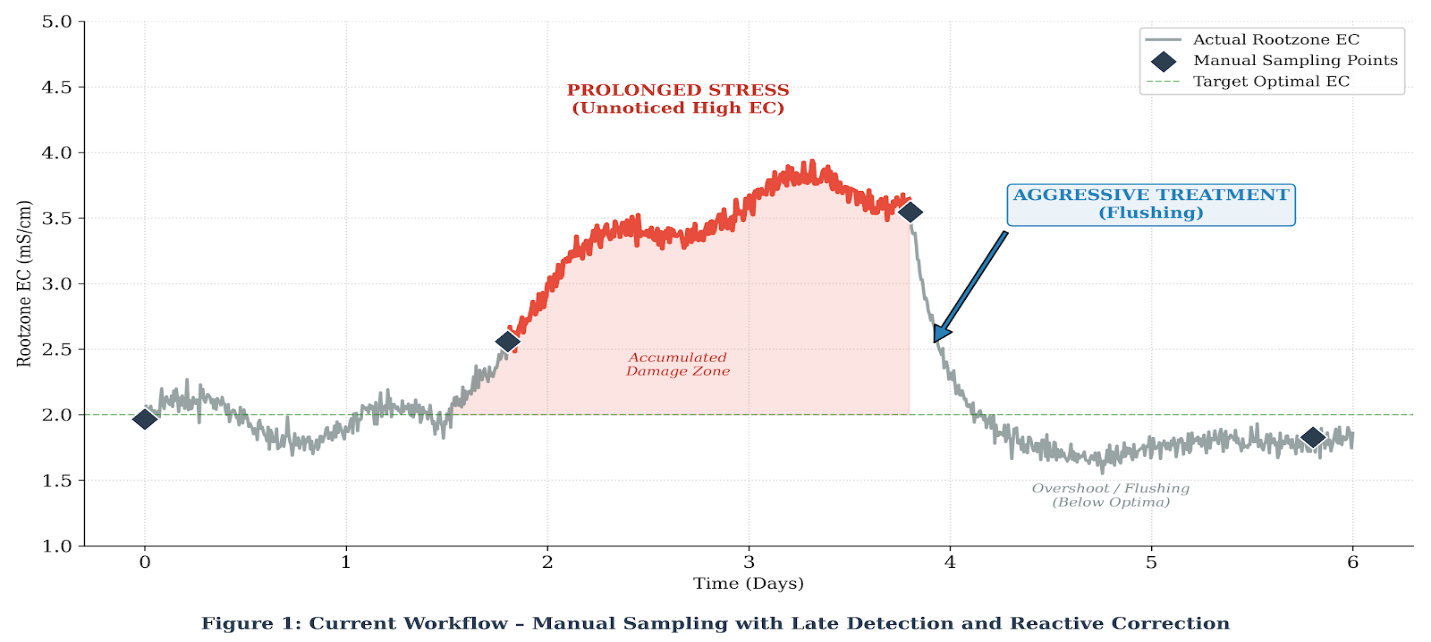
\includegraphics[width=0.92\textwidth]{figures/fig01.png}
    \caption{\LR{Current Workflow -- Manual Sampling with Late Detection and Reactive Correction}}
    \label{fig:workflow}
\end{figure}

איור \ref{fig:workflow} ממחיש תרחיש טיפוסי: מליחות בית השורשים חורגת מהטווח האופטימלי בין שתי דגימות ידניות, נשארת גבוהה לאורך פרק זמן ממושך ("אזור נזק מצטבר"), ומזוהה רק בדגימה המאוחרת -- מה שמחייב טיפול אגרסיבי (שטיפה) לתיקון המצב.

\textbf{חיישני קרקע רציפים \LR{(In-situ Sensors)}:} חיישנים אלו מספקים רצף נתונים \LR{(Time-Series)} ומאפשרים זיהוי מגמות בזמן אמת. אולם, השימוש בהם טומן בחובו אתגרים טכניים משמעותיים:

\begin{itemize}
    \item \textbf{סחיפה וכיול \LR{(Drift \& Calibration)}:} האלקטרודות נוטות לצבור משקעים וביופילם, הגורמים לקריאה "לנדוד" עם הזמן ולספק נתונים שגויים.
    \item \textbf{ייצוגיות מרחבית:} חיישן מודד נקודה בודדת במרחב. בחממה גדולה, או אפילו בתוך עציץ בודד, קיימת שונות מרחבית גבוהה ברטיבות ובמליחות. חיישן הממוקם ליד הטפטפת יראה ערך שונה לחלוטין מחיישן הממוקם בתחתית המצע.
    \item \textbf{עלות:} פריסה רחבה של חיישנים איכותיים דורשת השקעה כספית גבוהה ותחזוקה שוטפת.
\end{itemize}

\subsection{הבסיס הפיזיקלי-ביולוגי}
הקושי בחיזוי משתני השורשים נובע מכך שבית השורשים הוא מערכת דינמית המושפעת ממאזן מסה \LR{(Mass Balance)} משתנה. הצמח קולט מים ודשן בקצבים שונים:

\begin{itemize}
    \item \textbf{בימים של קרינה גבוהה:} הצמח מבצע דיות (Transpiration) מוגברת ו"שותה" בעיקר מים נקיים, מה שמותיר את המלחים במצע ועשוי לגרום לעליית EC מהירה.
    \item \textbf{בימים מעוננים:} קצב הדיות יורד, וצריכת המים והדשן מתאזנת.
\end{itemize}

המודל שלנו נועד ללמוד את הדפוסים הללו (הקשר הלא-ליניארי בין קרינה לצריכת מים) ולחזות את הצטברות המלחים שנובעת מהם.

\begin{figure}[H]
    \centering
    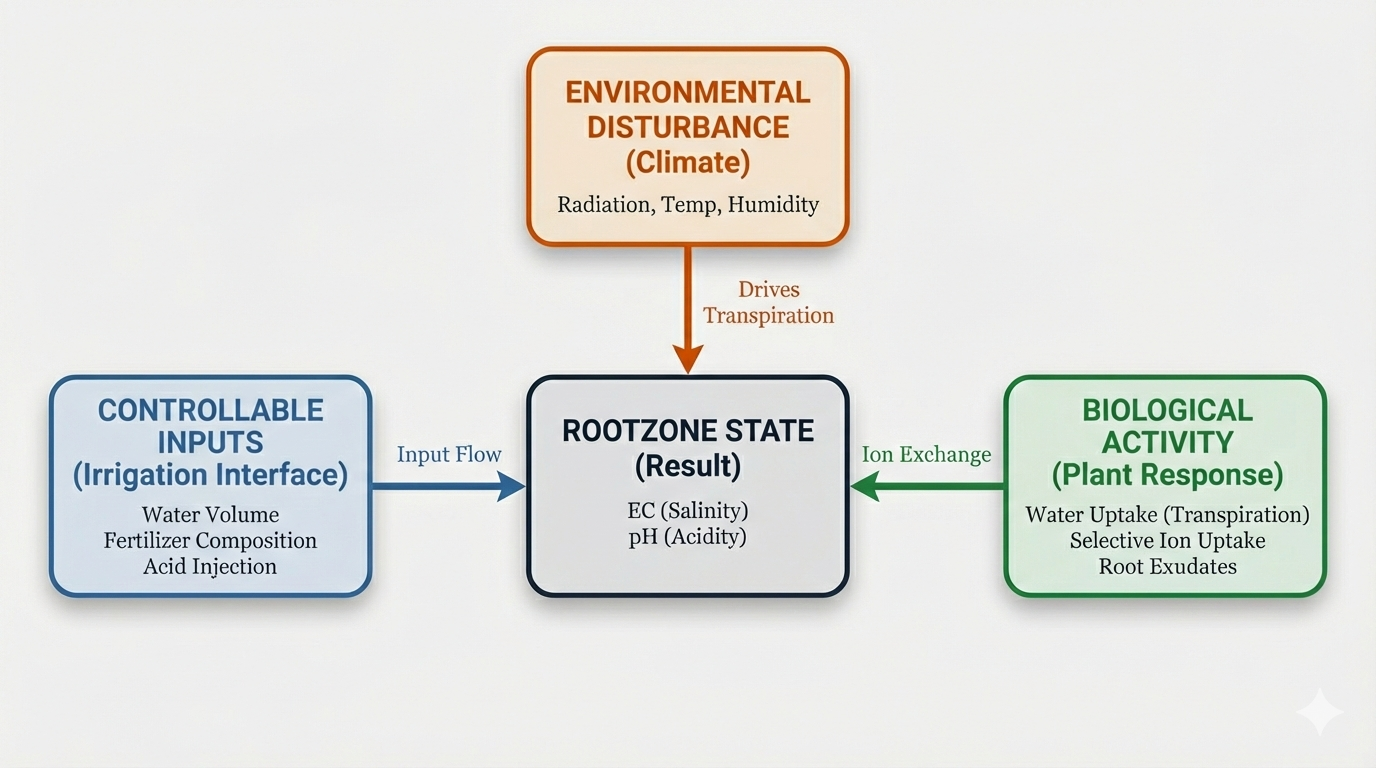
\includegraphics[width=0.85\textwidth]{figures/fig02.png}
    \caption{\LR{Physical-Biological Basis of Rootzone Dynamics}}
    \label{fig:physbio}
\end{figure}

כפי שמתואר באיור \ref{fig:physbio}, מצב בית השורשים הוא תוצאה של שילוב בין הפרעה סביבתית (אקלים, המניעה דיות), קלטים בני-שליטה (השקיה, דישון, חומצה) ופעילות ביולוגית של הצמח (קליטת מים וחילופי יונים).

\subsection{למה למידת מכונה?}
באופן מסורתי, ניתן לחזות תהליכים אלו באמצעות משוואות פיזיקליות מורכבות. אולם, מודלים אלו דורשים פרמטרים רבים שקשה מאוד למדוד בשטח (כגון מוליכות הידראולית של המצע, נקבוביות משתנה ושטח פנים של השורשים). גישת למידת המכונה \LR{(Data-Driven Approach)} עוקפת את הצורך במדידת הפרמטרים הללו. המודל אינו מחליף את ההבנה הפיזיקלית, אלא לומד קשרים אמפיריים מתוך הנתונים -- המודל לומד את ההתנהגות האפקטיבית של המערכת ישירות מתוך הנתונים ההיסטוריים, ובכך מאפשר דיוק גבוה בעלות חישובית נמוכה.

\subsection{הפתרון המוצע: "חיישן תוכנה" מבוסס נתונים}
פרויקט זה מציע גישה המבוססת על תפיסת ה־\LR{Soft Sensing} ("חיישן תוכנה"), שמטרתה להעריך את מצב בית השורשים גם בפרקי הזמן שבהם לא קיימת מדידה ישירה. ההנחה המרכזית היא שקיים קשר פיזיקלי-כימי בין תנאי הסביבה החיצוניים, המיקרו-אקלים בתוך החממה, פעולות המגדל כגון השקיה ודישון, ומדדי התגובה בבית השורשים.

באמצעות אלגוריתמים של למידת מכונה ניתן ללמוד קשרים מורכבים ובלתי ליניאריים אלו מתוך הנתונים ההיסטוריים, ולייצר תחזית של ערכי pH ו-EC על בסיס מידע זמין כגון נתוני אקלים, השקיה, דישון ומדידות עבר. גישה זו אינה מחליפה את המדידות הידניות המדויקות, אלא משלימה אותן ומסייעת לצמצם את פערי המידע בין מועדי הדגימה.

\subsection{מטרות הפרויקט}

\begin{itemize}
    \item \textbf{אינטגרציית נתונים:} יצירת מסד נתונים מאוחד \LR{(Master Dataset)} המשלב ומנרמל מקורות מידע הטרוגניים, ובהם נתוני אקלים חיצוני, נתוני מיקרו-אקלים בחממה, נתוני השקיה ודישון, משתני מצב הצמח ומדידות ידניות של pH ו-EC.
    \item \textbf{פיתוח מודל חיזוי לבית השורשים:} בניית מודל למידת מכונה המסוגל לחזות את ערכי ה-pH וה-EC בנקודת זמן עתידית, על בסיס מדידה נוכחית ידועה, תנאי הסביבה, פעולות ההשקיה והדישון, ומצב הצמח בפרק הזמן הרלוונטי. מטרת המודל היא לשמש כ־\SoftSensor{} המאפשר הערכת מצב רציפה יותר של בית השורשים בין מדידות ידניות דלילות.
    \item \textbf{שילוב בין למידה מדפוסים לבין חיזוי מגמות:} פיתוח גישה היברידית המשלבת מודל \GB{}, הלומד דפוסים מורכבים מתוך נתוני העבר, עם רכיב ליניארי חסין המסייע בהתמודדות עם אירועים תפעוליים חריגים או בעלי השפעה גבוהה. שילוב זה נועד לאפשר גם אינטרפולציה בתוך תחומי התנהגות מוכרים וגם אקסטרפולציה זהירה במצבים שבהם נדרשת תגובה לשינוי חד.
    \item \textbf{ולידציה בתנאי אמת:} בחינת ביצועי המודל באמצעות \WFV{} ובדיקות Holdout על מרווחים מדולגים, באופן המדמה תרחיש תפעולי שבו המודל מאומן על נתוני עבר ונדרש לחזות נקודות עתידיות. מטרת הוולידציה היא להעריך את יציבות המודל ואת התאמתו לשימוש ככלי תומך החלטה לניהול השקיה ודישון.
\end{itemize}

\section{הגדרת הבעיה}

\subsection{ניסוח הבעיה}
בגידולים אינטנסיביים על מצע מנותק, בית השורשים (Rootzone) הוא מערכת דינמית שקשה למדוד באופן רציף ומייצג. ערכי המוליכות החשמלית (EC) והחומציות (pH) מושפעים בו-זמנית מתנאי האקלים, מהמיקרו-אקלים בתוך החממה, ממשטר ההשקיה והדישון, ממצב הצמח ומהיסטוריית האירועים במצע. כתוצאה מכך, שינוי קטן באחד מגורמים אלו עשוי להוביל לשינוי משמעותי בסביבת השורשים.

הבעיה המרכזית במחקר נובעת מהפער בין הצורך בבקרה רציפה ומדויקת של בית השורשים לבין מגבלות אמצעי הניטור הקיימים כיום:

\begin{itemize}
    \item \textbf{מגבלת הניטור המקוטע:} בדיקות ידניות או בדיקות מעבדה של נקז/מצע מספקות מדידה מדויקת יחסית, אך הן דלילות בזמן ומייצגות נקודת זמן מסוימת בלבד. בין דגימה לדגימה עלולים להתרחש שינויים ברמת המליחות או החומציות, שאינם מתועדים בזמן אמת.
    \item \textbf{מגבלת החיישנים הרציפים:} חיישנים המוצבים במצע יכולים לספק סדרת זמן רציפה, אך הם רגישים לבעיות כיול, סחיפה, רעש וייצוגיות מרחבית. מאחר שהחיישן מודד נקודה אחת בלבד, ייתכן שהקריאה אינה מייצגת את מצב כלל בית השורשים.
    \item \textbf{ניהול תגובתי:} בהיעדר יכולת חיזוי, המגדל נדרש לעיתים להגיב לחריגות רק לאחר שהן כבר התרחשו. מצב זה מקשה על שמירה יציבה של תנאי בית השורשים ועלול להוביל לשימוש לא מיטבי במים, בדשן ובתיקוני חומציות.
\end{itemize}

לכן, הבעיה המחקרית היא כיצד ניתן להעריך את מצב בית השורשים בפרקי הזמן שבין המדידות הישירות, ולחזות את ערכי ה-pH וה-EC העתידיים על בסיס מידע זמין ממקורות אחרים.

\subsection{שאלת המחקר}
שאלת המחקר המרכזית היא:

\begin{quote}
\itshape
האם ניתן לפתח מודל למידת מכונה המסוגל לחזות את ערכי ה-pH וה-EC בבית השורשים בנקודת זמן עתידית, על בסיס מדידה נוכחית ידועה, נתוני אקלים ומיקרו-אקלים, נתוני השקיה ודישון, מצב הצמח והיסטוריית המדידות?
\end{quote}

מתוך שאלה זו נגזרות שאלות משנה:

\begin{itemize}
    \item \textbf{דיוק החיזוי:} מהי רמת הדיוק שניתן להשיג בחיזוי ערכי pH ו-EC, כאשר ההערכה מתבססת על מדדי השגיאה MAE ו-RMSE ועל מדד ההסבר \Rtwo{}, והאם דיוק זה מתאים לשימוש ככלי תומך החלטה?
    \item \textbf{תרומת המשתנים:} אילו קבוצות משתנים תורמות באופן המשמעותי ביותר לחיזוי השינויים בבית השורשים: תנאי אקלים, השקיה, דישון, מצב הצמח, מדידות עבר או משך הזמן בין המדידה הנוכחית לנקודת החיזוי?
    \item \textbf{יציבות לאורך זמן:} האם המודל שומר על ביצועים יציבים כאשר הוא נבחן בשיטת ולידציה קדימה בזמן, המדמה תרחיש שבו המודל מאומן על נתוני עבר ונדרש לחזות נקודות עתידיות?
    \item \textbf{יכולת הכללה:} האם המודל מצליח לשמור על רמת דיוק טובה גם בבדיקת הכללה על מרווחים מדולגים, שאינם משמשים לאימון המודל?
\end{itemize}

\subsection{השערת המחקר}
השערת המחקר היא שקיים קשר פיזיקלי-כימי ואגרונומי בין תנאי הסביבה, פעולות ההשקיה והדישון, מצב הצמח והשינויים בערכי ה-pH וה-EC בבית השורשים. קשר זה אינו בהכרח ליניארי, והוא עשוי לכלול השהיות, תגובות מצטברות ואירועים נקודתיים בעלי השפעה גבוהה.

בהתאם לכך, ההשערה היא שמודל למידת מכונה יוכל ללמוד את דפוסי התגובה של בית השורשים מתוך נתוני העבר, ולחזות את ערכי ה-pH וה-EC בנקודות זמן עתידיות. בפרט, משוער כי מודל היברידי, המשלב בין \GB{} ללמידת דפוסים מורכבים לבין רכיב ליניארי להתמודדות עם מגמות ואירועים חריגים, יוכל לשמש כ־\SoftSensor{} אמין יחסית, המשלים את המדידות הידניות ומצמצם את פערי המידע ביניהן.

\section{מושגים בסיסיים}
לצורך הבנת העבודה, להלן הסבר על המושגים המרכזיים בתחומי האגרונומיה, חיזוי סדרות עיתיות ולמידת מכונה שבהם נעשה שימוש בפרויקט.

\subsection{מושגים אגרונומיים}

\begin{itemize}
\item \textbf{\color{ruppinblue}מוליכות חשמלית \LR{(EC -- Electrical Conductivity)}:} מדד לכמות המלחים המומסים בתמיסת המצע או הקרקע. בחקלאות, EC משמש כאינדיקציה לרמת המליחות ולריכוז הדשן הזמין לצמח. ערכים גבוהים מדי עלולים לגרום לעקה אוסמוטית ולהקשות על קליטת מים, בעוד שערכים נמוכים מדי עשויים להעיד על מחסור בהזנה. המדד נמדד ביחידות mS/cm.

\item \textbf{\color{ruppinblue}חומציות \LR{(pH)}:} מדד לרמת החומציות או הבסיסיות של התמיסה. ערך ה-pH משפיע על מסיסות וזמינות יסודות ההזנה לצמח, ובפרט על זמינות מיקרו-אלמנטים כגון ברזל, מנגן ואבץ. סטייה מטווח ה-pH הרצוי עלולה לגרום למחסורי הזנה או לרעילות, גם כאשר הדשן סופק בכמות מספקת.

\item \textbf{\color{ruppinblue}התאדות-דיות \LR{(ET0 -- Evapotranspiration)}:} מדד המייצג את פוטנציאל איבוד המים מהמערכת כתוצאה מהתאדות ומהדיות של הצמח. ET0 מושפע בעיקר מקרינה, טמפרטורה, לחות ורוח, והוא משמש להערכת דרישת המים של הגידול ולתכנון השקיה.

\item \textbf{\color{ruppinblue}בית שורשים \LR{(Rootzone)}:} נפח המצע או הקרקע שבו מתפתחת מערכת השורשים של הצמח. באזור זה מתרחשים תהליכי קליטת מים ודשן, הצטברות מלחים ושינויים בחומציות. לכן, תנאי בית השורשים משפיעים ישירות על בריאות הצמח, קצב הצימוח והיבול.

\item \textbf{\color{ruppinblue}מצע מנותק:} שיטת גידול שבה הצמח גדל במצע שאינו הקרקע הטבעית, כגון קוקוס, פרלייט או מצעים מלאכותיים אחרים. במצע מנותק נפח בית השורשים מוגבל וקיבולת הבאפר נמוכה יחסית, ולכן שינויים בהשקיה, בדישון או במליחות עשויים להשפיע במהירות על הצמח.
\end{itemize}

\subsection{מושגים בלמידת מכונה}

\begin{itemize}
\item \textbf{\color{ruppinblue}מודל רגרסיה \LR{(Regression Model)}:} מודל חיזוי שמטרתו להעריך ערך מספרי רציף. בפרויקט זה נעשה שימוש במודלי רגרסיה לצורך חיזוי ערכי pH ו-EC, וכן לצורך חיזוי משתני מיקרו-אקלים בתוך החממה.

\item \textbf{\color{ruppinblue}חיישן תוכנה \LR{(Soft Sensor)}:} מודל חיזוי המשמש להערכת משתנה שקשה או יקר למדוד באופן רציף, על בסיס משתנים אחרים שקל יותר למדוד. בפרויקט זה, ה־\SoftSensor{} נועד להעריך את ערכי ה-pH וה-EC בבית השורשים בין מועדי המדידה הידניים, באמצעות נתוני אקלים, השקיה, דישון, מצב הצמח ומדידות עבר.

\item \textbf{\color{ruppinblue}\GB{}:} משפחת אלגוריתמים המבוססת על שילוב הדרגתי של עצי החלטה רבים. כל עץ חדש נבנה במטרה לתקן את השגיאות של העצים הקודמים, וכך מתקבל מודל חיזוי חזק המסוגל ללמוד קשרים מורכבים ולא ליניאריים בין משתנים.

\item \textbf{\color{ruppinblue}\LR{XGBoost}:} מימוש מתקדם ויעיל של \GB{} המבוסס על עצי החלטה. האלגוריתם מתאים במיוחד לנתונים טבלאיים, מאפשר למידה של קשרים לא-ליניאריים, ומתמודד היטב עם שילובים מורכבים בין משתנים. בפרויקט זה שימש XGBoost כרכיב המרכזי במודל החיזוי של בית השורשים.

\item \textbf{\color{ruppinblue}\LR{LightGBM}:} אלגוריתם נוסף ממשפחת \GB{} המתאפיין במהירות אימון גבוהה וביעילות חישובית. בפרויקט זה שימש LightGBM בעיקר בשלבי חיזוי משתני מיקרו-אקלים בתוך החממה, על בסיס נתוני אקלים חיצוני.

\item \textbf{\color{ruppinblue}מודל ליניארי חסין \LR{(Robust Linear Model)}:} מודל רגרסיה ליניארי שנועד להיות פחות רגיש לערכים חריגים ולרעש בנתונים. בפרויקט זה שולב רכיב ליניארי חסין כחלק מהמודל ההיברידי, במטרה לשפר את תגובת החיזוי במצבים של אירועים תפעוליים בעלי השפעה גבוהה, כגון שינוי חד במליחות או מעבר בין מגמות.

\item \textbf{\color{ruppinblue}מודל היברידי:} מודל המשלב יותר מגישת חיזוי אחת. בפרויקט זה המודל ההיברידי משלב בין \GB{}, הלומד דפוסים מורכבים מתוך נתוני העבר, לבין רכיב ליניארי חסין, המסייע בהתמודדות עם מגמות ואירועים חריגים. שילוב זה מאפשר למודל לבצע גם אינטרפולציה בתוך דפוסים מוכרים וגם אקסטרפולציה זהירה במצבים פחות שכיחים.

\item \textbf{\color{ruppinblue}אינטרפולציה:} חיזוי עבור מצב הדומה למצבים שכבר הופיעו בנתוני האימון. לדוגמה, חיזוי תגובת בית השורשים ביום בעל תנאי אקלים והשקיה הדומים לימים שנצפו בעבר.

\item \textbf{\color{ruppinblue}אקסטרפולציה:} חיזוי עבור מצב החורג חלקית מהדפוסים שנצפו בנתוני האימון. בפרויקט זה מושג זה רלוונטי בעיקר לאירועים תפעוליים חריגים או לשינויים חדים במליחות ובחומציות, שבהם נדרש מהמודל להעריך מגמת שינוי גם מעבר לדוגמאות השכיחות בנתונים.

\item \textbf{\color{ruppinblue}\WFV{}:} שיטת אימות המתאימה לסדרות עיתיות. במקום לחלק את הנתונים באופן אקראי לאימון ולבדיקה, המודל מאומן על נתוני העבר ונבדק על נקודות עתידיות. לאחר מכן נקודת הזמן מתקדמת, והמודל נבחן שוב. שיטה זו מדמה תרחיש תפעולי שבו בכל שלב זמינים רק נתוני העבר.

\item \textbf{\color{ruppinblue}\LR{Holdout}:} שיטת בדיקה שבה חלק מהנתונים נשמר מחוץ לתהליך האימון ומשמש להערכת ביצועי המודל לאחר האימון. בפרויקט זה נעשה שימוש גם בבדיקת Holdout על מרווחים מדולגים, כדי לבחון האם המודל מסוגל לחזות נקודות שלא שימשו ללמידה.

\item \textbf{\color{ruppinblue}הנדסת פיצ'רים \LR{(Feature Engineering)}:} תהליך יצירת משתנים חדשים מתוך הנתונים הגולמיים במטרה לשפר את יכולת הלמידה של המודל. דוגמאות מפרויקט זה הן זמן שעבר מאז ההשקיה האחרונה, סכום הקרינה המצטבר, כמות הדשן בפרק זמן נתון, משך הזמן בין מדידת הבסיס לנקודת החיזוי, ומדדי היסטוריה של בית השורשים.

\item \textbf{\color{ruppinblue}\LR{MAE -- Mean Absolute Error}:} מדד שגיאה המחושב כממוצע הערכים המוחלטים של ההפרשים בין הערכים האמיתיים לערכים החזויים. ככל שה-MAE נמוך יותר, כך החיזוי מדויק יותר. היתרון המרכזי של MAE הוא שהוא נמדד באותן יחידות של המשתנה החזוי, למשל יחידות pH או mS/cm עבור EC.

\item \textbf{\color{ruppinblue}\LR{RMSE -- Root Mean Squared Error}:} מדד שגיאה המחושב כשורש ממוצע ריבועי השגיאות. RMSE נותן משקל גבוה יותר לשגיאות גדולות, ולכן הוא מתאים לזיהוי מצבים שבהם המודל מבצע טעויות חריגות.

\item \textbf{\color{ruppinblue}\Rtwo{} (מקדם ההסבר):} מדד המבטא איזה חלק מהשונות בנתוני היעד מוסבר על ידי המודל. ערך הקרוב ל-1 מעיד על התאמה טובה יותר של המודל לנתונים, בעוד שערך נמוך מעיד כי המודל מתקשה להסביר את השונות.
\end{itemize}

\section{סקירת ספרות}

השימוש במודלים מבוססי נתונים \LR{(Data-Driven Models)} בחקלאות מדייקת צבר תאוצה בשנים האחרונות, ומאפשר להחליף מדידות פיזיקליות יקרות באמצעות אלגוריתמים המעבדים נתוני סביבה ותפעול. עם זאת, יישום מודלים אלו במערכות דינמיות כמו חממות מחייב התמודדות עם אירועי קצה חריגים כגון קפיצות מליחות או צניחת pH. אתגר זה דורש מהמודל לא רק לחזות בדיוק מצבי שגרה מוכרים (אינטרפולציה), אלא גם לבצע אקסטרפולציה אמינה מחוץ לטווח הנתונים ההיסטורי.

כדי להתמודד עם אתגר זה, סקירה זו משלבת שני צירי ספרות: הראשון בוחן יישומי למידה עמוקה לחיזוי משתני קרקע בחקלאות, והשני מתמקד בספרות האלגוריתמית הבוחנת את מגבלות עצי ההחלטה, ומבססת את הצורך בארכיטקטורה היברידית המשלבת רכיב ליניארי למצבי קיצון.

אחד האתגרים המרכזיים בגידול בחממות הוא השליטה ברמת המליחות (EC) בבית השורשים. במחקרם של \LR{Moon et al.\ (2018)} בחנו החוקרים את היכולת לחזות את ה-EC של תמיסת ההזנה במערכות הידרופוניות סגורות \LR{(Closed-loop soilless cultures)}. החוקרים השתמשו ברשת נוירונים מסוג RNN \LR{(Recurrent Neural Network)} ובפרט במודל LSTM הידוע ביכולתו ללמוד סדרות עיתיות. המחקר הראה כי שילוב של משתני אקלים (קרינה, טמפרטורה ולחות יחסית) יחד עם נתוני תפעול (כמות השקיה וריכוז דשן במי ההשקיה), מאפשר לחזות בדיוק רב את ה-EC העתידי במצע. המסקנה המרכזית ממחקר זה, הרלוונטית לעבודתנו, היא שקיים קשר הדוק וניתן למידול בין עומס האקלים החיצוני לבין הדינמיקה הכימית בבית השורשים, וכי היסטוריית הנתונים \LR{(Time-lagged features)} היא קריטית לביצועי המודל.

בעוד ש-Moon התמקד בכימיה של המים, \LR{Lü et al.\ (2025)} הציגו גישה מתקדמת לחיזוי רטיבות קרקע בבית השורשים \LR{(RZSM -- Root Zone Soil Moisture)}. המחקר התמודד עם הקושי למדוד רטיבות בעומק הקרקע והציע מודל היברידי המשלב מודל פיזיקלי הידרולוגי (Hydrus-1D) עם מודל למידה עמוקה מסוג CNN-LSTM-Attention. המחקר הדגים כיצד מודלים של למידה עמוקה \LR{(Deep Learning)} יכולים ללמוד את הקשרים הלא-ליניאריים המורכבים בין רטיבות פני השטח (הניתנת למדידה קלה או חישה מרחוק) לבין המתרחש בעומק בית השורשים. השימוש במנגנון קשב \LR{(Attention Mechanism)} אפשר למודל להתמקד בטווחי הזמן המשפיעים ביותר על המצב הנוכחי. אף על פי שמחקר זה בוצע בתנאי שדה \LR{(Oasis field)} ולא בחממה, הוא מחזק את ההנחה כי ניתן לייצר "חיישן וירטואלי" לתנאי עומק הקרקע על בסיס נתונים סביבתיים, וכי שילוב של ארכיטקטורות המביאות בחשבון את המימד הרציף של הזמן כגון LSTM או נגזרותיו משפר משמעותית את הדיוק בהשוואה למודלים סטטיים.

לצד היתרונות של מודלים אלו במצבי שגרה, הציר השני בספרות מתמקד בבחירת ארכיטקטורת האלגוריתם המתאימה להתמודדות עם חריגות מהדפוסים המוכרים. במחקרם של \LR{Muckley et al.\ (2023)} נבחנה שאלת האקסטרפולציה במודלים מדעיים מבוססי למידת מכונה. החוקרים השוו בין מודלים מורכבים מסוג \LR{Random Forest} ורשתות נוירונים לבין מודלים ליניאריים פשוטים, תוך התמקדות בבעיות מתחום מדעי החומרים. ממצאי המחקר הראו כי מודלים מורכבים נוטים להציג ביצועים טובים יותר במצבי אינטרפולציה, שבהם הדוגמאות החדשות נמצאות בתוך תחום הנתונים שנלמד. לעומת זאת, כאשר נדרשה אקסטרפולציה מעבר לטווח הנתונים, המודלים הליניאריים הפשוטים היו תחרותיים מאוד ולעיתים אף הציגו ביצועים טובים יותר -- ממצא התומך בשילוב רכיב ליניארי במצבים שבהם המערכת חורגת מהדפוסים הרגילים.

לעומת זאת, במחקרם של \LR{Loh et al.\ (2007)} הוצגה תמונה זהירה וממוקדת יותר לגבי אקסטרפולציה בסביבת עצים. החוקרים בחנו עצי מודל ליניאריים \LR{(Linear Model Trees)}, כלומר עצים שבהם בכל עלה מותאם מודל ליניארי מקומי, והראו כי אף על פי שמבנה כזה מאפשר למודל להמשיך מגמות מעבר לטווח הנתונים, הוא עלול גם ליצור שגיאות גדולות (קטסטרופליות) כאשר ההנחה הליניארית מופעלת רחוק מדי ממרכז הנתונים בעלה הספציפי. ממצא זה מדגיש כי רכיב ליניארי אינו צריך להחליף את המודל המרכזי, אלא לפעול בזהירות, באופן מוגבל ומבוקר, ומצדיק שימוש במודלים משלימים רובסטיים כגון רגרסיית הובר \LR{(Huber Regressor)} הניחנת בעמידות גבוהה בפני תצפיות חריגות (Outliers).

גישה המחזקת תפיסה היברידית זו מופיעה במחקרם של \LR{Friedberg et al.\ (2021)}, שבו הוצע לשלב בין \LR{Random Forest} לבין התאמה ליניארית מקומית \LR{(Local Linear Forests)}. החוקרים ציינו כי יערות אקראיים הם מודלים חזקים וגמישים ללמידת קשרים לא-ליניאריים, אך יש להם מגבלה מובנית בתיאור אותות חלקים ומגמות רציפות \LR{(Continuous trends)}. כדי להתמודד עם מגבלה זו, הם שילבו את מנגנון החלוקה של היער עם רגרסיה ליניארית מקומית, כך שהמודל שומר על היתרון של עצים בזיהוי אזורים ודפוסים, אך מוסיף יכולת טובה יותר לתיאור מגמות רציפות. באופן דומה, במחקרם של \LR{Cai et al.\ (2023)} הוצע מודל בשם \LR{Extrapolated Random Tree for Regression} שמטרתו לשפר את יכולת האקסטרפולציה של עצי רגרסיה באמצעות שילוב מנגנון אקסטרפולציה המבוסס על רגרסיה ליניארית בתוך מבנה העץ, ובכך הוכח כי שילוב רכיב אקסטרפולטיבי משפר משמעותית את ביצועי המודל מחוץ לטווח המוכר.

הספרות הקיימת מצביעה על היתכנות גבוהה לשימוש בלמידת מכונה לניטור בית השורשים. בעוד ש-Moon et al.\ התמקדו ב-EC ו-Lü et al.\ ברטיבות, פרויקט זה שואף לשלב גישות אלו ולפתח מודל אחוד החוזה הן את ה-EC והן את ה-pH, תוך שימוש באלגוריתמים של למידת מכונה מבוססי עצים המציעים איזון בין דיוק ליכולת פרשנות ומתאימים ליישום במערכות בקרה תפעוליות בחממות מסחריות. יחד עם זאת, לאור מגבלות האקסטרפולציה של מודלים מורכבים במצבי קצה, כפי שעולה ממחקריהם של Muckley, Loh, Friedberg ו-Cai, הפרויקט אינו נשען על אלגוריתם בודד. תחת זאת, מיושמת גישה היברידית: שימוש באלגוריתמים מבוססי-עצים המציעים איזון בין דיוק ליכולת פרשנות במצבי שגרה, בשילוב רכיב ליניארי מבוקר המבטיח יציבות באירועים חריגים. שילוב זה מייצר מודל שלם ואמין, המותאם ליישום מעשי במערכות בקרה תפעוליות בחממות מסחריות.

\begin{figure}[H]
    \centering
    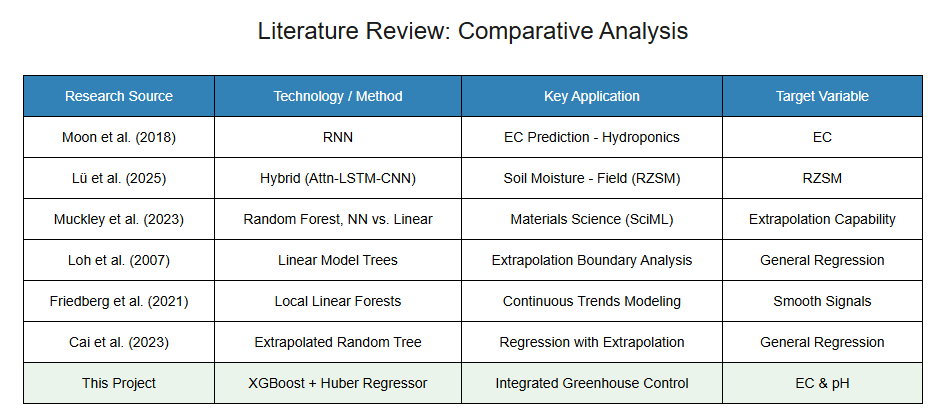
\includegraphics[width=\textwidth]{figures/fig03.png}
    \caption{\LR{Literature Review -- Comparative Analysis of Related Methods}}
    \label{fig:litreview}
\end{figure}

איור \ref{fig:litreview} מסכם את המחקרים שנסקרו, את השיטות שבהן נעשה שימוש, את יישומם המרכזי ואת המשתנה החזוי, לצד מיקומו של פרויקט זה במרחב זה.

\section{גישת הפתרון}

כדי להתמודד עם האתגר של חיזוי משתנים ביו-כימיים מורכבים בבית השורשים, פותחה גישה מערכתית המבוססת על שרשרת חיזוי דו-שלבית. גישה זו מפרקת את הבעיה לשני שלבים מרכזיים: תחילה חיזוי ותיאור תנאי המיקרו-אקלים בתוך החממה, ולאחר מכן חיזוי תגובת בית השורשים על בסיס תנאים אלו, פעולות ההשקיה והדישון, מצב הצמח ומדידות עבר.

מבנה זה מאפשר להשתמש בנתונים זמינים יחסית, כגון אקלים חיצוני, השקיה, דישון ומדידות ידניות קודמות, כדי להעריך את ערכי ה-pH וה-EC גם בפרקי הזמן שבהם לא קיימת מדידה ישירה של בית השורשים.

\subsection{מסד הנתונים}
המחקר מתבסס על נתונים אגרו-מטאורולוגיים ותפעוליים שנאספו במהלך עונת הגידול 2025, בין החודשים מאי לספטמבר. לצורך אימון ובדיקת המודלים נבנה מסד נתונים מאוחד (Master) המשלב מקורות מידע הטרוגניים לאחר תהליכי ניקוי, סנכרון ואיחוד לזמן אחיד.

מסד הנתונים הסופי נבנה ברזולוציה של 10 דקות וכלל 16{,}682 רשומות, בטווח התאריכים 29.05.2025 עד 21.09.2025. הנתונים נחלקים לשתי קבוצות עיקריות:

\begin{itemize}
    \item \textbf{נתונים רציפים:} נתונים שנמדדו בתדירות גבוהה ממקורות כגון תחנה מטאורולוגית חיצונית ולוגר נתונים פנימי בחממה. נתונים אלו כוללים משתנים כגון קרינה, טמפרטורה, לחות יחסית, מהירות רוח, טמפרטורת קרקע והתאדות פוטנציאלית.
    \item \textbf{נתונים בדידים ודלילים:} מדידות ידניות של ערכי pH ו-EC בבית השורשים. מדידות אלו משמשות כערכי היעד של המודל, אך הן דלילות ביחס לנתוני האקלים והתפעול. בסך הכול היו 109 נקודות מדידה מתויגות של pH ו-EC.
\end{itemize}

פער זה בין נתונים רציפים וצפופים לבין מדידות יעד דלילות היווה את אחד האתגרים המרכזיים בפרויקט. לכן, המודל לא נבנה כחיזוי פשוט של כל נקודת זמן, אלא כחיזוי שינוי בין נקודת בסיס ידועה $t_0$ שבה קיימת מדידת pH ו-EC לבין נקודת יעד עתידית $t_1$.

\subsection{השלמת נתונים היסטוריים \LR{(Data Imputation using LightGBM)}}
אחד האתגרים בפרויקט היה חוסר רציפות בחלק מנתוני המיקרו-אקלים בתוך החממה. כדי להימנע מאובדן תקופות שבהן קיימות מדידות בית שורשים אך חסרים נתוני אקלים פנימי, פותחו מודלים לחיזוי משתני מיקרו-אקלים על בסיס נתוני אקלים חיצוניים.

מודלים אלו למדו את הקשר בין תנאי האקלים מחוץ לחממה לבין התנאים בתוך החממה, כגון טמפרטורה, לחות, קרינה פנימית והתאדות. בדרך זו ניתן היה להשלים או לחזות משתנים פנימיים הדרושים למודל בית השורשים, ולהגדיל את כמות המידע הזמין עבור שלב החיזוי המרכזי.

\begin{figure}[H]
    \centering
    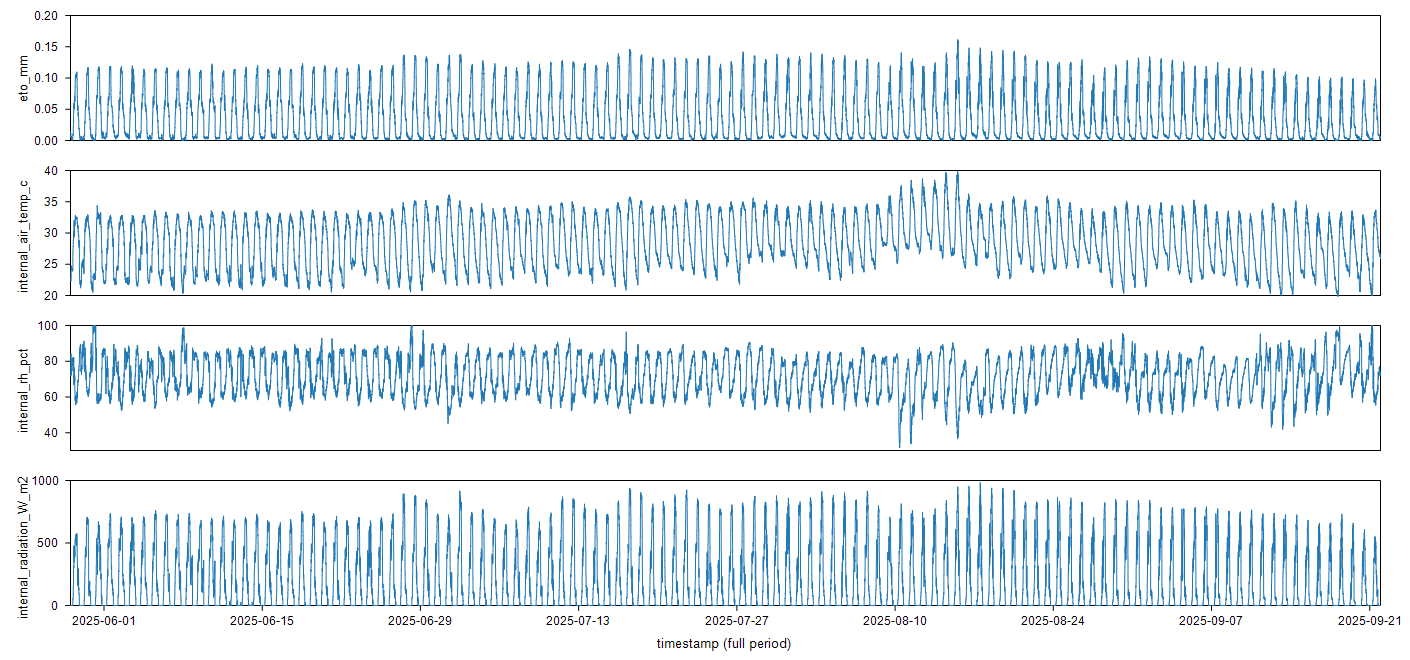
\includegraphics[width=\textwidth]{figures/fig04.png}
    \caption{\LR{Historical Microclimate Data Imputation Results}}
    \label{fig:imputation}
\end{figure}

איור \ref{fig:imputation} מציג את סדרות הזמן של משתני המיקרו-אקלים (ET0, טמפרטורה פנימית, לחות יחסית וקרינה פנימית) לאורך כל תקופת הניסוי, לאחר תהליך ההשלמה.

\subsection{עיבוד מקדים}
לפני שלב האימון בוצע עיבוד מקדים לנתונים, שכלל ניקוי ערכים חריגים או לא פיזיקליים, טיפול בחוסרים, וסנכרון זמני המדידה בין מקורות המידע השונים.

בנוסף, לכל מרווח חיזוי בין $t_0$ ל-$t_1$ הוצמדה היסטוריית התנאים שהתרחשה בין שתי הנקודות. כלומר, עבור כל דגימת יעד של pH ו-EC חושבו משתני אקלים, השקיה, דישון ומצב צמח המתארים את התהליך שהוביל מהמצב ההתחלתי למצב העתידי.

\subsection{ארכיטקטורת המערכת}
המערכת בנויה כשני שלבים עיקריים:

\textbf{שלב 1: מודל מיקרו-אקלים.} שלב זה נועד לתרגם את תנאי האקלים החיצוניים לתנאים הצפויים בתוך החממה. המודל מקבל כקלט משתנים כגון קרינה, טמפרטורה, לחות ומהירות רוח, ומפיק הערכה של משתני מיקרו-אקלים פנימיים, כגון טמפרטורה, לחות, קרינה פנימית והתאדות. הרציונל הוא שבית השורשים מושפע מהתנאים בתוך החממה ולא רק מתנאי הסביבה החיצונית. לכן, שלב זה מאפשר להשתמש במידע מטאורולוגי זמין כבסיס לחיזוי מדויק יותר של סביבת הגידול בפועל.

\textbf{שלב 2: מודל בית השורשים.} זהו מודל הליבה של הפרויקט. המודל מקבל כקלט את ערכי ה-pH וה-EC בנקודת הבסיס, את תנאי המיקרו-אקלים, את נתוני ההשקיה והדישון, את מצב הצמח ואת משך הזמן בין $t_0$ ל-$t_1$. על בסיס מידע זה הוא חוזה את ערכי ה-pH וה-EC בנקודת הזמן העתידית.

בשלב הסופי פותח מודל היברידי, המשלב בין רכיב \GB{} לבין רכיב ליניארי חסין. רכיב ה־\GB{} נועד ללמוד דפוסים מורכבים ולא ליניאריים מתוך נתוני העבר, בעוד שהרכיב הליניארי מסייע בהתמודדות עם מגמות ואירועים תפעוליים בעלי השפעה גבוהה. שילוב זה מאפשר למודל לבצע גם אינטרפולציה בתוך דפוסים מוכרים וגם אקסטרפולציה זהירה במצבים חריגים יותר.

\begin{figure}[H]
    \centering
    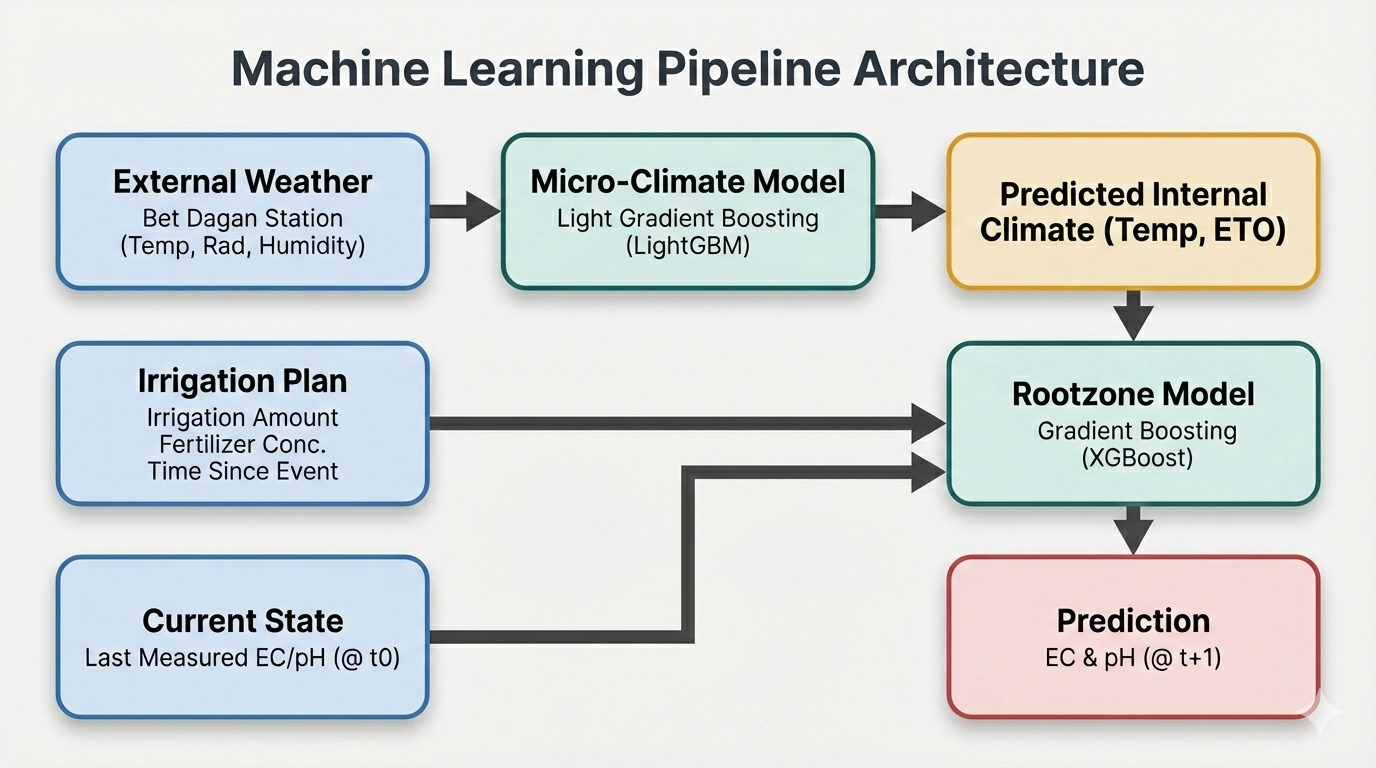
\includegraphics[width=0.8\textwidth]{figures/fig06.png}
    \caption{\LR{System Architecture -- Two-Stage Prediction Architecture}}
    \label{fig:architecture}
\end{figure}

איור \ref{fig:architecture} ממחיש את זרימת המידע בין שני השלבים: נתוני מזג האוויר החיצוני עוברים דרך מודל המיקרו-אקלים (LightGBM), ותוצאתו, יחד עם תוכנית ההשקיה והמצב ההתחלתי, מוזנת למודל בית השורשים (XGBoost) המפיק את התחזית הסופית.

\subsection{אסטרטגיית איחוד הנתונים}
אחד האתגרים המרכזיים בפרויקט היה השוני ברזולוציית הזמן בין מקורות הנתונים. נתוני האקלים והלוגר נאספו בתדירות גבוהה של 10 דקות, בעוד שמדידות pH ו-EC בוצעו באופן ידני ובתדירות נמוכה בהרבה.

כדי להתמודד עם פער זה, נבנה \LR{Master Dataset} בציר זמן אחיד של 10 דקות. הנתונים הרציפים נשמרו ברזולוציה המקורית, ואילו מדידות ה-pH וה-EC שימשו כנקודות יעד בלבד. מודל בית השורשים אומן על מרווחים שבהם קיימת מדידת בסיס ומדידת יעד, ולא על כל נקודת זמן בנפרד.

\begin{figure}[H]
    \centering
    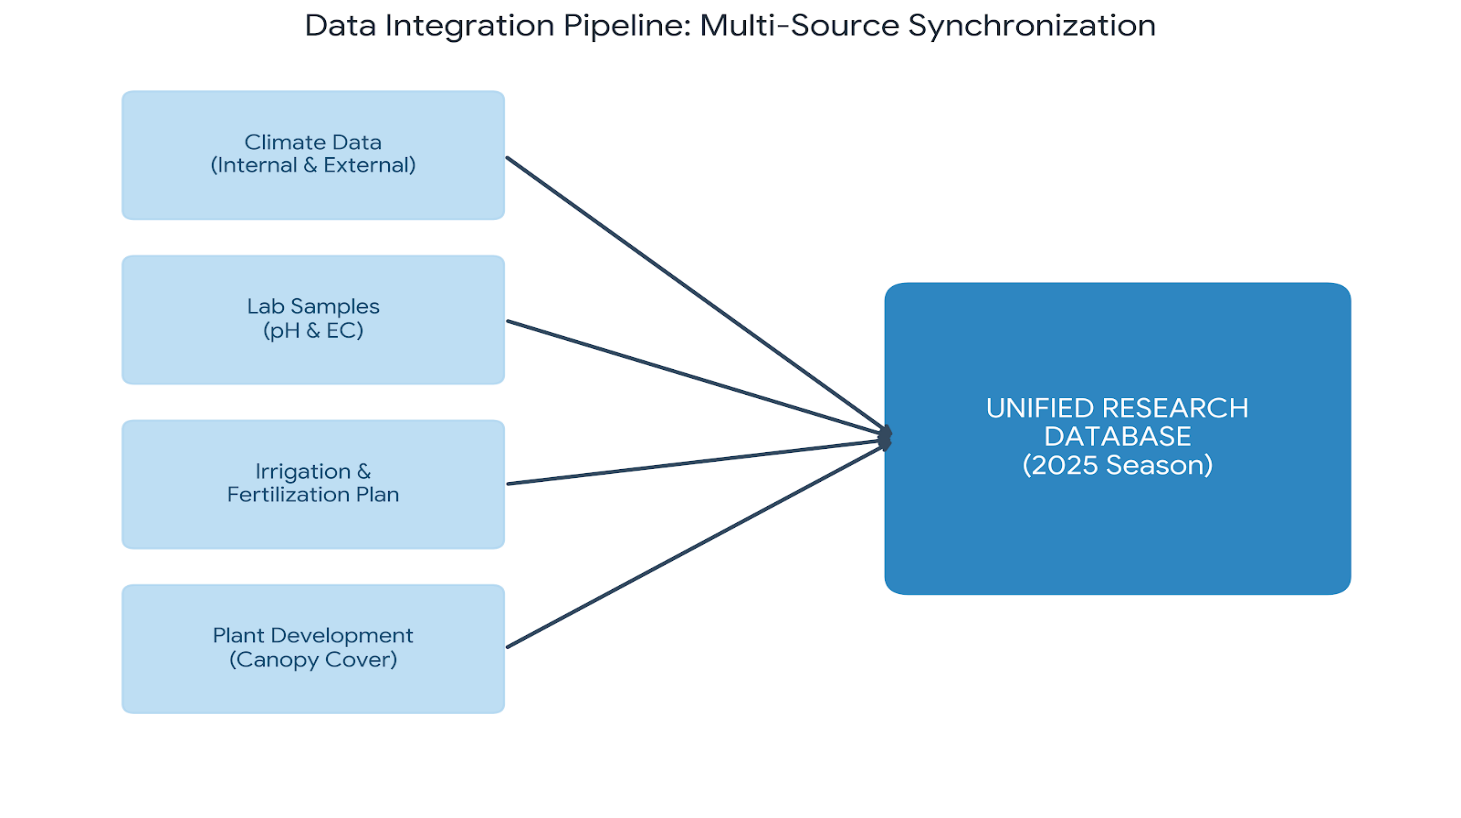
\includegraphics[width=0.8\textwidth]{figures/fig05.png}
    \caption{\LR{Data Integration Pipeline -- Unified Master Dataset Construction}}
    \label{fig:pipeline}
\end{figure}

גישה זו, המתוארת באיור \ref{fig:pipeline}, מאפשרת למודל ללמוד את השינוי שהתרחש בבית השורשים לאורך מרווח זמן נתון, במקום לנסות לחזות ערך רגעי ללא מדידת אמת תואמת.

\subsection{הנדסת פיצ'רים \LR{(Feature Engineering)}}
כדי לאפשר למודל ללמוד את התהליכים האגרונומיים והפיזיקליים המשפיעים על בית השורשים, נבנו משתנים חדשים מתוך הנתונים הגולמיים.

\begin{itemize}
    \item \textbf{משתני מצב התחלתי:} ערכי pH ו-EC בנקודת הבסיס $t_0$ המשמשים כעוגן לחיזוי.
    \item \textbf{משתני אופק חיזוי:} משך הזמן בין נקודת הבסיס לנקודת היעד, המבטא את פרק הזמן שבו הצטברו השפעות האקלים, ההשקיה והדישון.
    \item \textbf{משתני צבירה:} סכומי קרינה, התאדות, השקיה ודישון בפרקי זמן שונים. משתנים אלו מייצגים את "הזיכרון" המצטבר של המערכת.
    \item \textbf{משתני אירועים:} זמן מאז השקיה, דישון או אירוע תפעולי אחר. משתנים אלו חשובים לזיהוי תגובות מושהות של בית השורשים.
    \item \textbf{משתני מצב הצמח:} כיסוי נוף וגיל הצמח, המשמשים כאינדיקציה לגודל הצמח, קצב הדיות וצריכת המים והדשן.
\end{itemize}

\subsection{אסטרטגיית אימון ובדיקה \LR{(Walk-Forward Validation)}}
מאחר שהנתונים הם סדרה עיתית, לא נעשה שימוש בחלוקה אקראית רגילה לסט אימון וסט בדיקה, כדי למנוע זליגת מידע מהעתיד לעבר. במקום זאת יושמה שיטת \WFV{}.

בשיטה זו, המודל מאומן בכל שלב על נתוני העבר בלבד ונבחן על נקודות עתידיות. לאחר מכן חלון האימון מתקדם בזמן, והמודל נבחן שוב. תהליך זה מדמה תרחיש תפעולי שבו בכל נקודת זמן זמינים למודל רק הנתונים שנאספו עד אותה נקודה.

\begin{figure}[H]
    \centering
    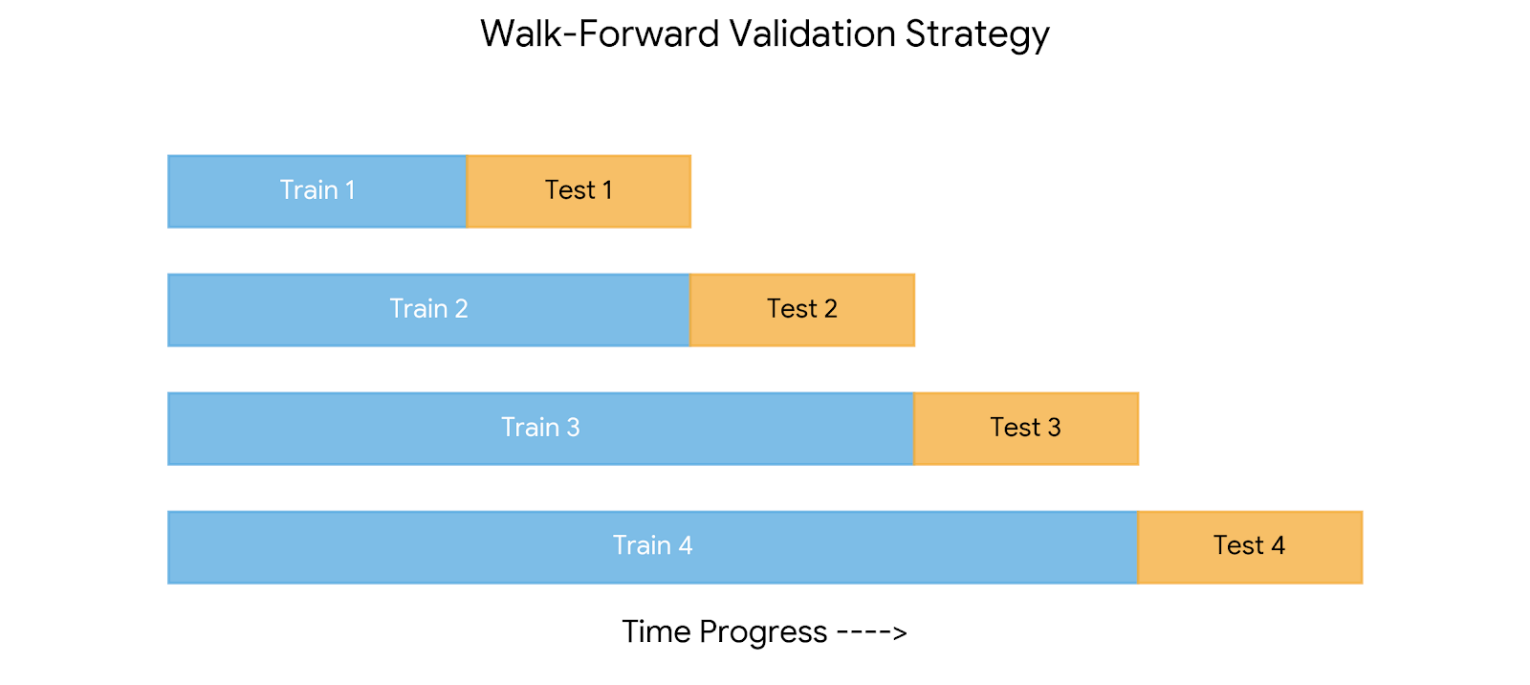
\includegraphics[width=0.8\textwidth]{figures/fig07.png}
    \caption{\LR{Walk-Forward Validation Strategy}}
    \label{fig:walkforward}
\end{figure}

כפי שמתואר באיור \ref{fig:walkforward}, בכל איטרציה מתרחב חלון האימון, ואילו חלון הבדיקה מתקדם בזמן -- כך שהמודל תמיד נבחן על נתונים עתידיים ביחס לחלון האימון שלו.

בנוסף, בוצעה בדיקת Holdout על מרווחים מדולגים, שבה חלק מהמרווחים הוצאו מתהליך האימון ושימשו לבדיקת יכולת ההכללה של המודל. בדיקה זו נועדה לבחון האם המודל מסוגל לחזות נקודות שלא שימשו ללמידה, ולא רק לשחזר דפוסים מתוך נתוני האימון.

בפרויקט נבחנו גרסאות חיזוי שונות, ובהן גרסת 24 שעות וגרסת 48 שעות. הגרסה הסופית מדגישה את יכולת המודל לחזות את תגובת בית השורשים בטווח של עד 48 שעות, תוך שמירה על מבנה בדיקה המדמה שימוש עתידי במערכת תומכת החלטה.

\section{תוצאות ואתגרים}

\subsection{תוצאות המודלים}
בשלב הסופי של הפרויקט נבחנה המערכת על נתוני עונת הגידול 2025, בטווח החודשים מאי--ספטמבר. המערכת כוללת שני רכיבים מרכזיים: מודל מיקרו-אקלים, המשמש להערכת תנאי הסביבה בתוך החממה, ומודל בית שורשים, החוזה את ערכי ה-pH וה-EC על בסיס מדידה נוכחית, תנאי סביבה, השקיה, דישון ומצב הצמח.

\subsubsection*{א. מודל המיקרו-אקלים}
המודל הציג רמת דיוק גבוהה בחיזוי משתני המיקרו-אקלים המרכזיים:

\begin{itemize}
    \item \textbf{טמפרטורה פנימית:} התקבל דיוק גבוה מאוד, עם מקדם הסבר של כ-\Rtwo{}=0.97 ושגיאה ממוצעת של פחות מ-0.8 מעלות צלזיוס.
    \item \textbf{לחות יחסית:} התקבל מקדם הסבר של כ-\Rtwo{}=0.87, עם שגיאה ממוצעת של כ-2.5 אחוזי לחות.
    \item \textbf{התאדות פוטנציאלית \LR{(ET0)}:} התקבל דיוק גבוה, עם \Rtwo{} של כ-0.97 ושגיאה מוחלטת ממוצעת של כ-0.016 מ"מ.
    \item \textbf{קרינה פנימית:} הקרינה בתוך החממה חושבה ונחזתה על בסיס נתוני הקרינה החיצונית ותנאי המבנה, ומהווה משתנה מרכזי להערכת עומס האנרגיה על הצמח, קצב הדיות והצטברות מלחים במצע.
    \item \textbf{טמפרטורת קרקע:} טמפרטורת הקרקע שימשה כמשתנה משלים לתיאור סביבת בית השורשים, מכיוון שהיא משפיעה על פעילות השורשים, זמינות יסודות ההזנה וקצב התהליכים הכימיים והביולוגיים במצע.
\end{itemize}

משמעות תוצאות אלו היא שמודל המיקרו-אקלים יכול לשמש שכבת קלט אמינה למודל בית השורשים. כלומר, ניתן להשתמש בו כמעין "תחנה מטאורולוגית וירטואלית" בתוך החממה.

\begin{table}[H]
    \centering
    \begin{LTR}
    \begin{tabular}{lccc}
        \toprule
        \textbf{Target Variable} & \textbf{MAE} & \textbf{\Rtwo{}} & \textbf{RMSE} \\
        \midrule
        Internal Air Temp (\textdegree C) & 0.431 & 0.972 & 0.580 \\
        Internal RH (\%)                  & 2.72  & 0.861 & 3.56  \\
        Internal Radiation                & 22.47 & 0.966 & 43.97 \\
        ET0                               & 0.0035 & 0.973 & 0.0059 \\
        Soil Temp (\textdegree C)         & 0.857 & 0.921 & 1.19  \\
        \bottomrule
    \end{tabular}
    \end{LTR}
    \caption{\LR{Overall Micro-Climate Model Performance}}
    \label{tab:microclimate}
\end{table}

\begin{figure}[H]
    \centering
    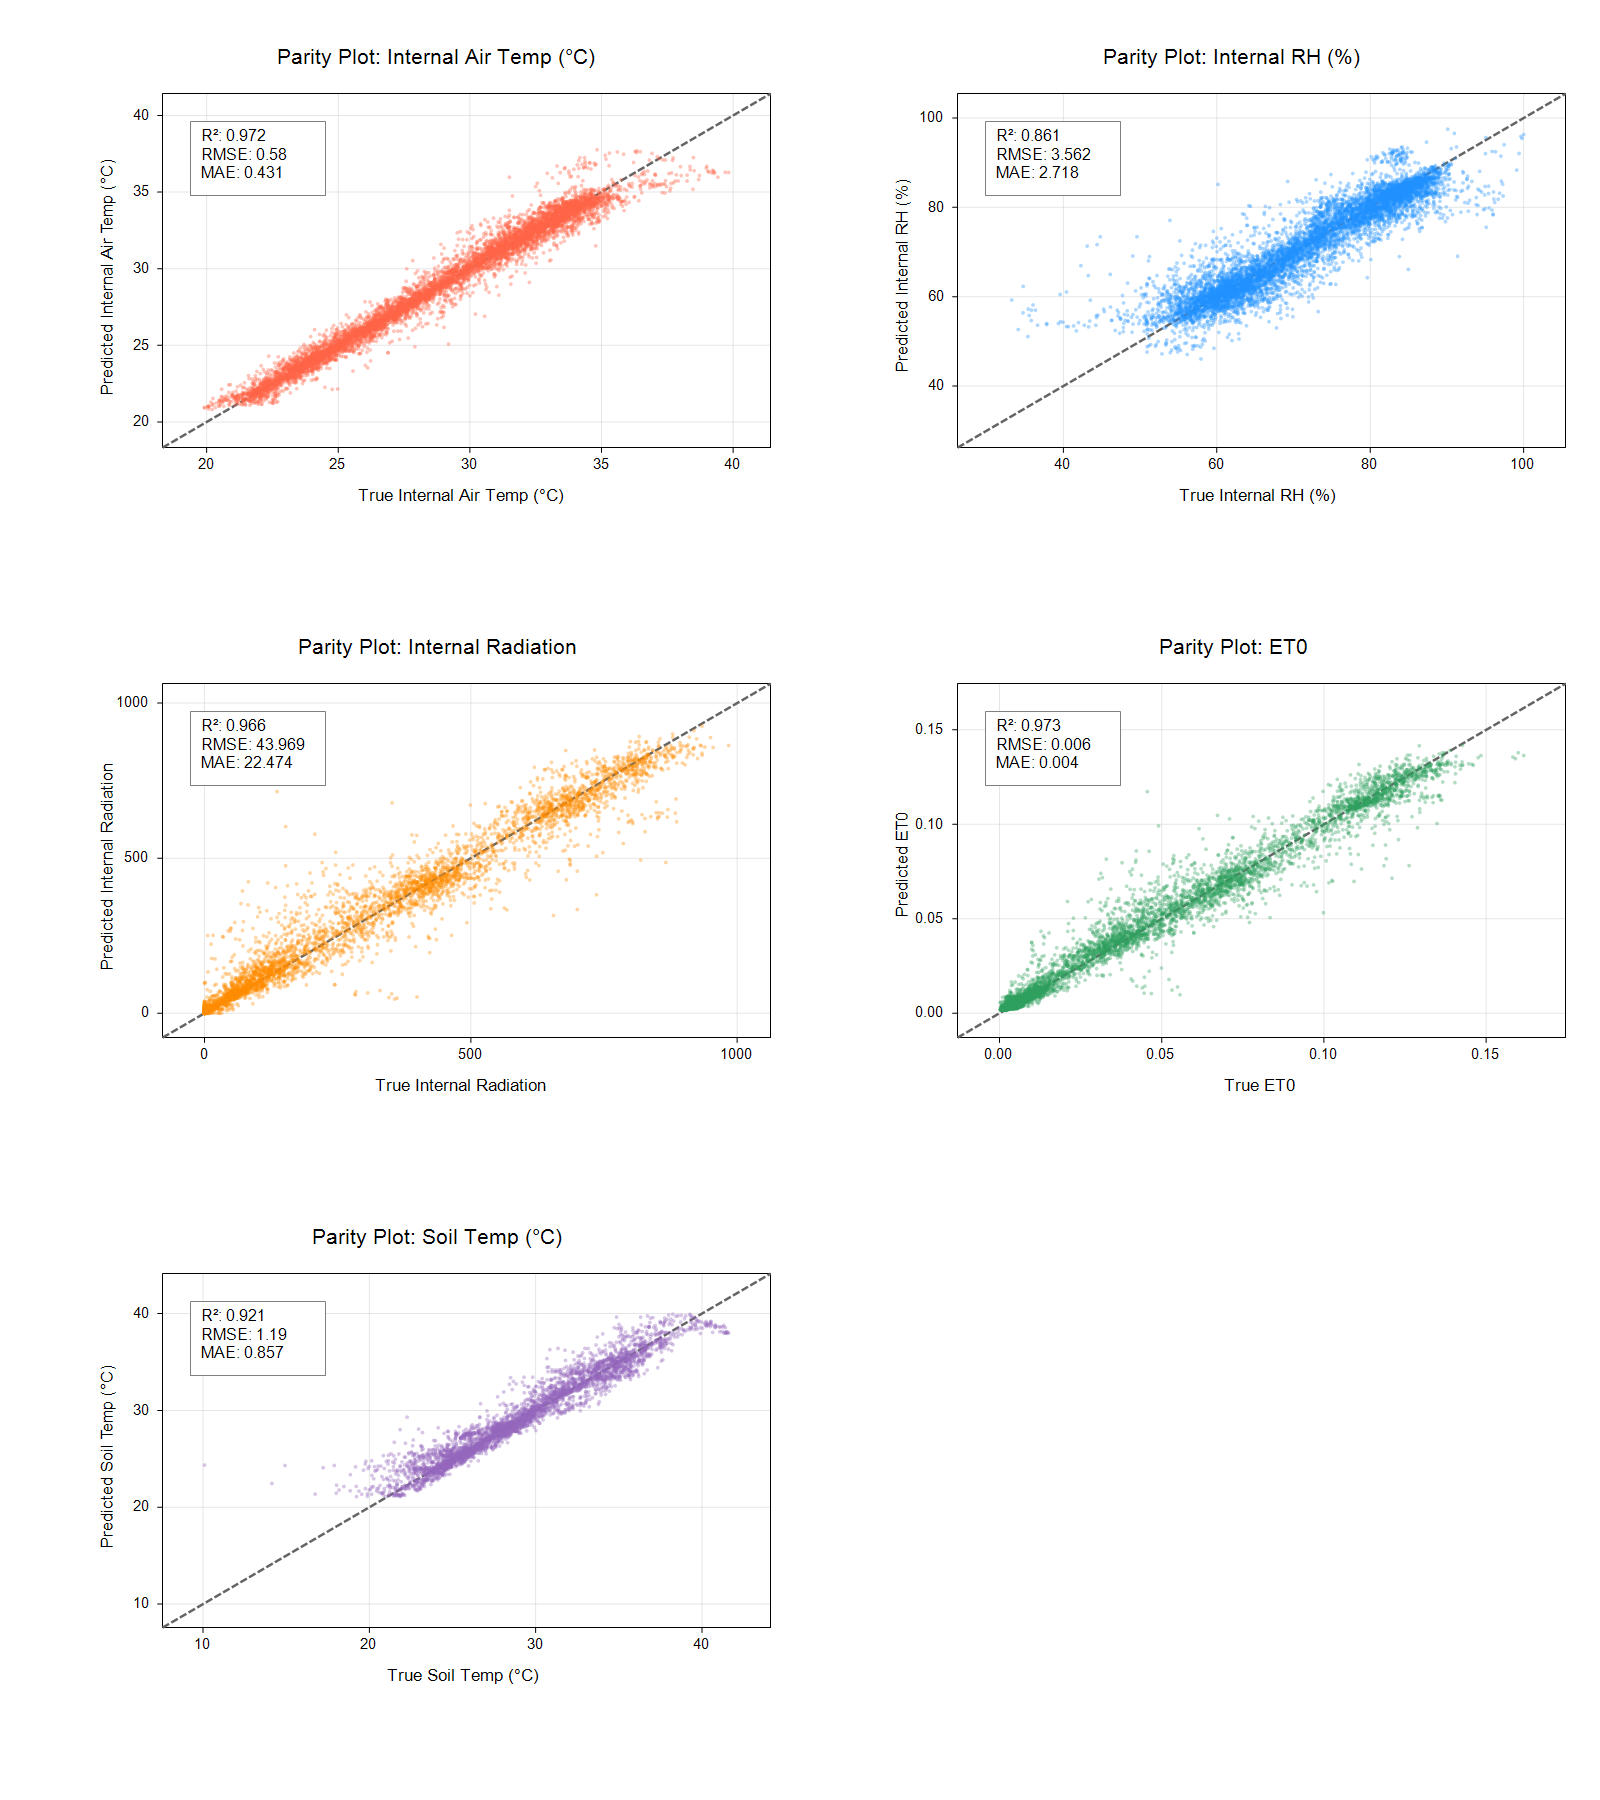
\includegraphics[width=\textwidth]{figures/fig08.png}
    \caption{\LR{Microclimate Model Results -- Parity Plot}}
    \label{fig:parity}
\end{figure}

\subsubsection*{ב. מודל בית השורשים}
מודל בית השורשים הוא מודל החיזוי המרכזי בפרויקט. המודל נבחן באמצעות \WFV{}, המדמה תרחיש שבו המודל מאומן על נתוני עבר בלבד ונדרש לחזות נקודות עתידיות. בנוסף, בוצעה בדיקת Holdout על מרווחים מדולגים, במטרה לבחון את יכולת ההכללה של המודל.

עבור pH המודל הציג ביצועים יציבים וטובים. במבחן Walk-Forward התקבלה שגיאת MAE של כ-0.33 יחידות pH, ובמבחן Holdout התקבלה שגיאת MAE של כ-0.29 יחידות pH. ערך ה-\Rtwo{} עמד על כ-0.93, והמודל שיפר את החיזוי בכ-62\% ביחס למודל נאיבי המבוסס על שמירת הערך האחרון שנמדד.

עבור EC התקבלה שגיאת MAE של כ-0.127 mS/cm במבחן Walk-Forward וכ-0.131 mS/cm במבחן Holdout. ערכי ה-\Rtwo{} היו גבוהים: כ-0.98 במבחן Walk-Forward וכ-0.95 במבחן Holdout. ביחס למודל נאיבי, התקבל שיפור של כ-35\% בדיוק החיזוי.

תוצאות אלו מצביעות על כך שהמודל מצליח ללמוד את הדינמיקה של בית השורשים מתוך שילוב של נתוני אקלים, השקיה, דישון, מצב הצמח ומדידות עבר. עם זאת, חיזוי EC נותר מאתגר יותר מחיזוי pH, בעיקר בטווחי מוליכות נמוכים שבהם גם שגיאה אבסולוטית קטנה מתורגמת לשגיאה יחסית גבוהה.

\begin{figure}[H]
    \centering
    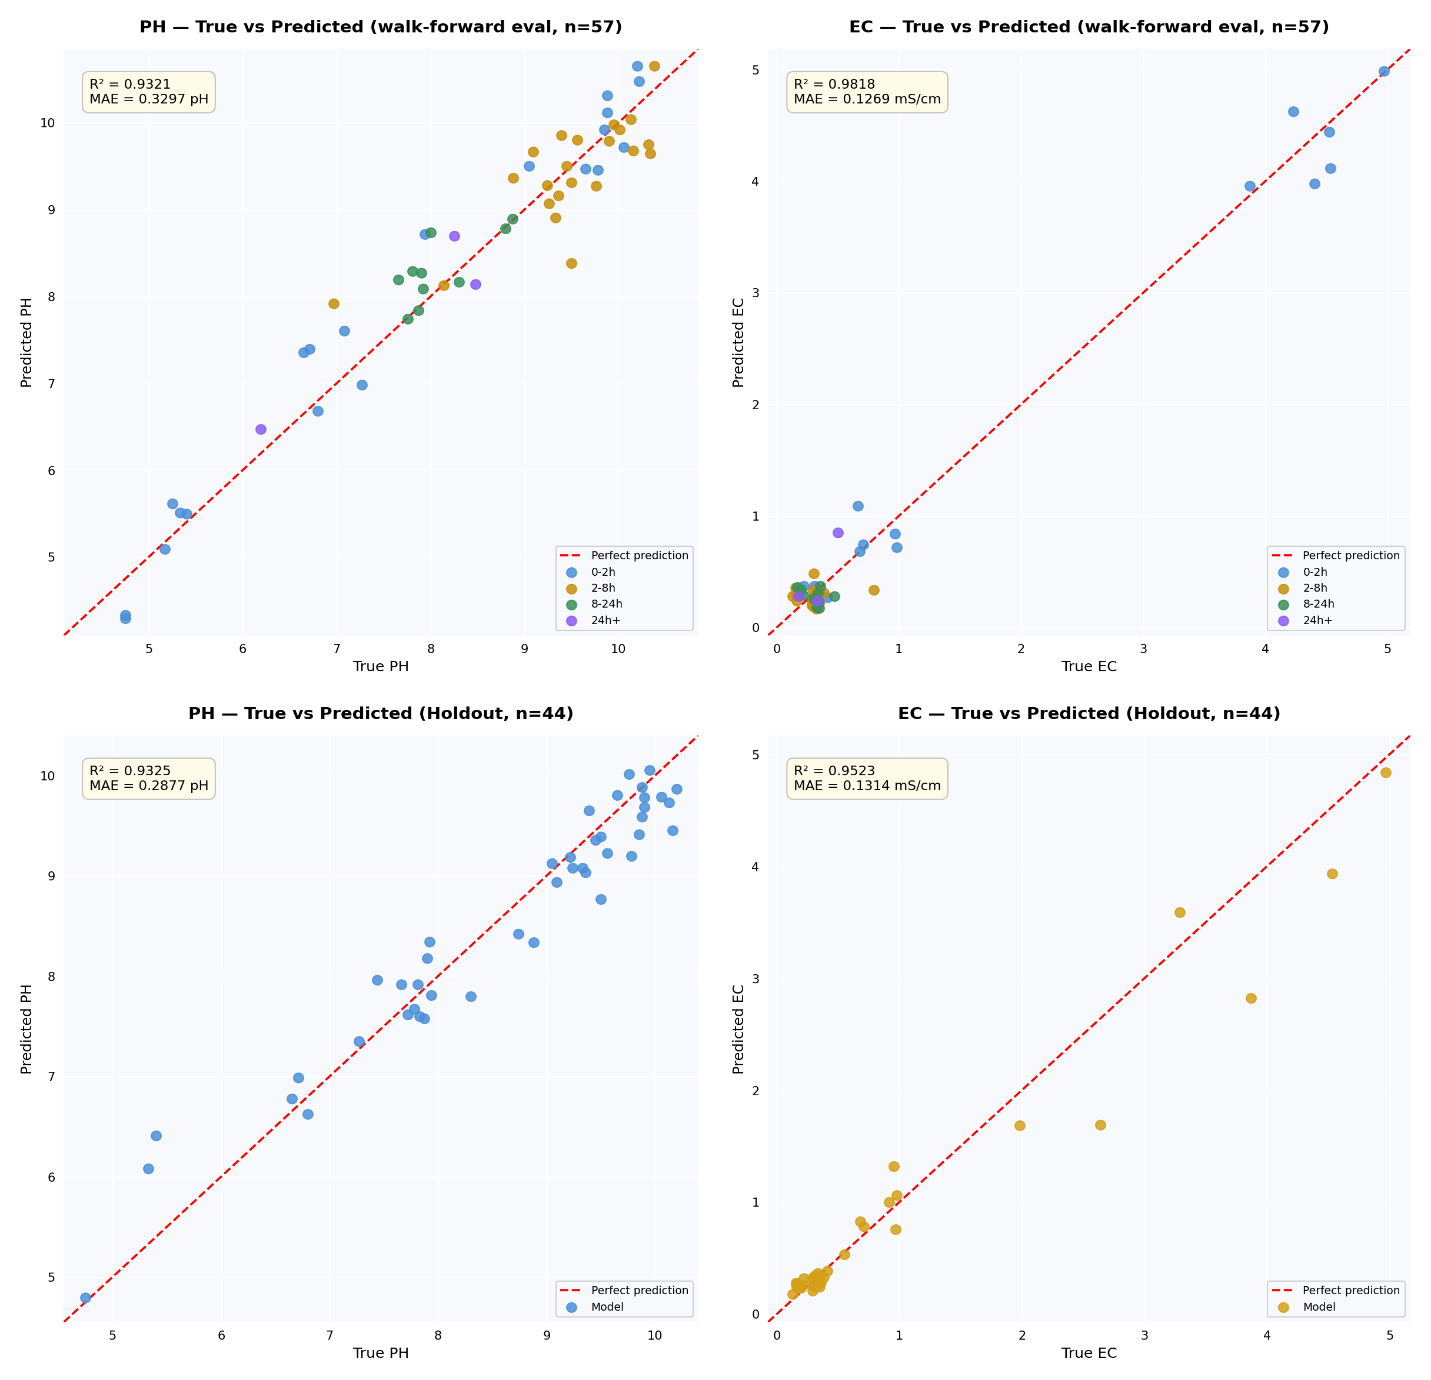
\includegraphics[width=\textwidth]{figures/fig09.png}
    \caption{\LR{Rootzone Model Results -- Scatter Plot}}
    \label{fig:scatter}
\end{figure}

\begin{table}[H]
    \centering
    \begin{LTR}
    \begin{tabular}{llccc}
        \toprule
        \textbf{Evaluation} & \textbf{Target Variable} & \textbf{MAE} & \textbf{\Rtwo{}} & \textbf{RMSE} \\
        \midrule
        Walk-Forward & pH          & 0.330 & 0.932 & 0.414 \\
        Walk-Forward & EC (mS/cm)  & 0.127 & 0.982 & 0.171 \\
        Holdout      & pH          & 0.288 & 0.933 & 0.360 \\
        Holdout      & EC (mS/cm)  & 0.131 & 0.952 & 0.255 \\
        \bottomrule
    \end{tabular}
    \end{LTR}
    \caption{\LR{Rootzone Model Performance: Walk-Forward and Holdout}}
    \label{tab:rootzone_metrics}
\end{table}

\begin{figure}[H]
    \centering
    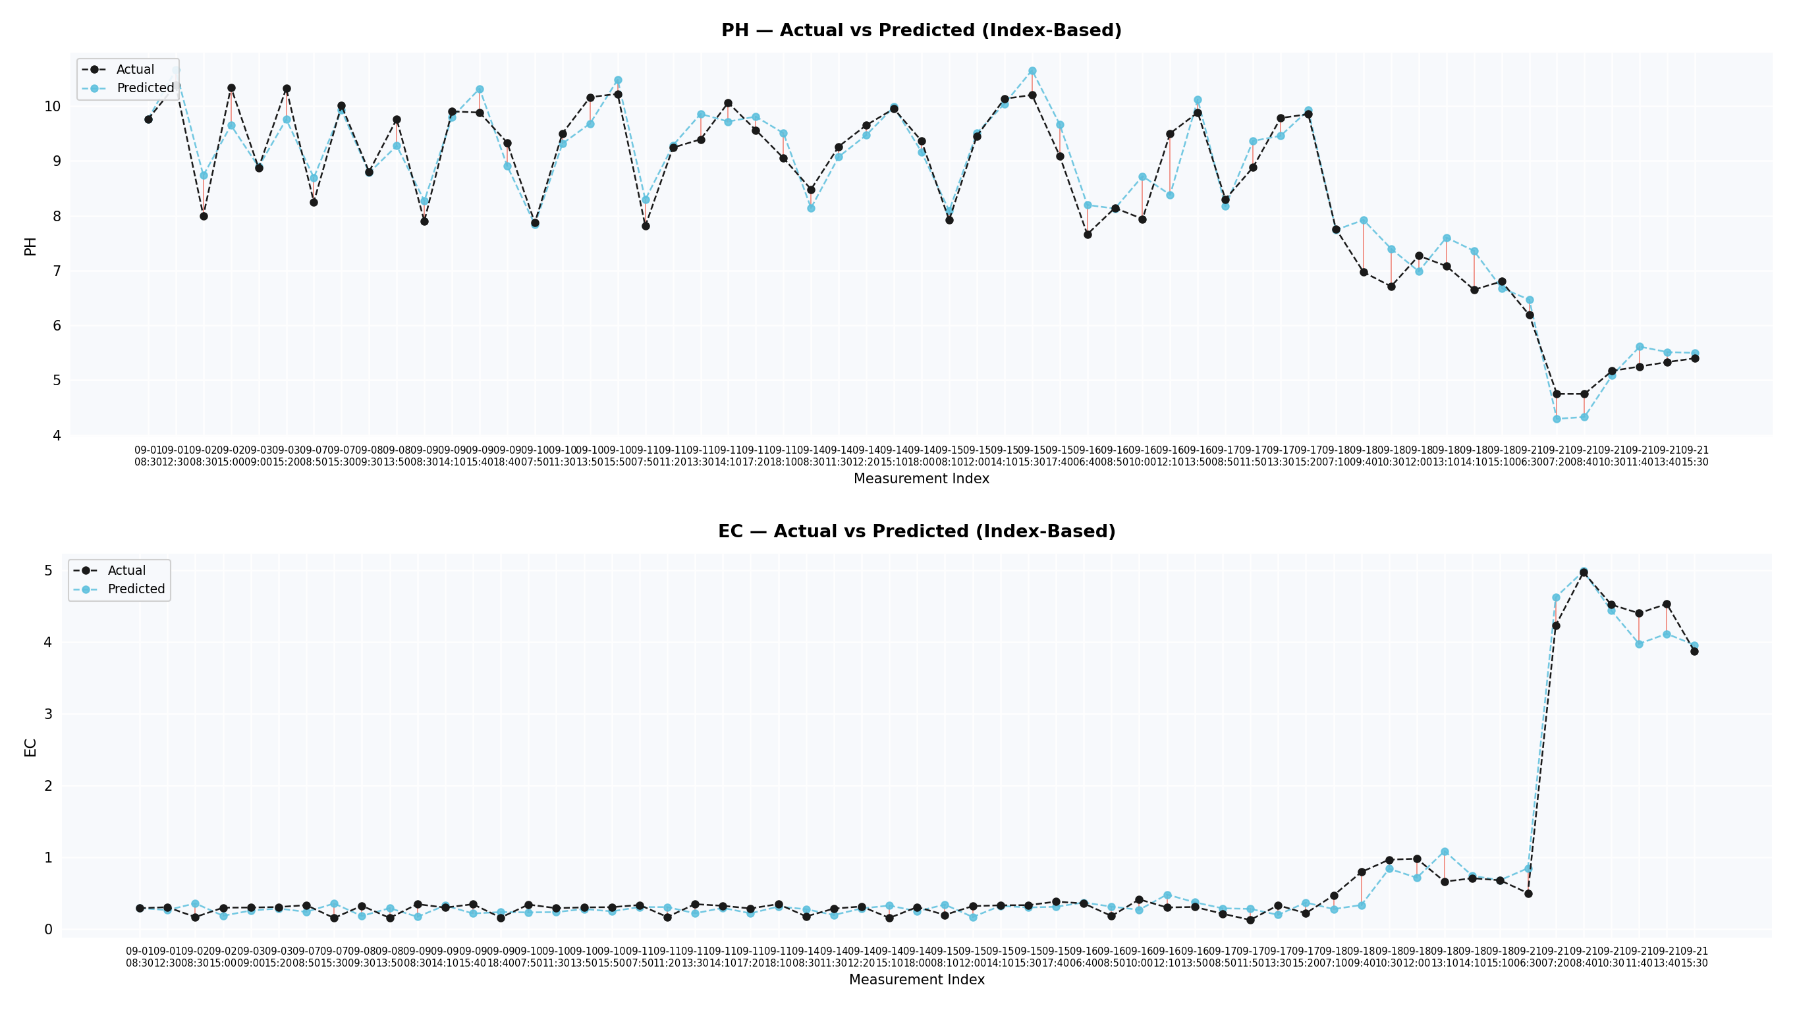
\includegraphics[width=\textwidth]{figures/fig10.png}
    \caption{\LR{Rootzone Model Results -- Time-Series Prediction}}
    \label{fig:timeseries}
\end{figure}

\begin{figure}[H]
    \centering
    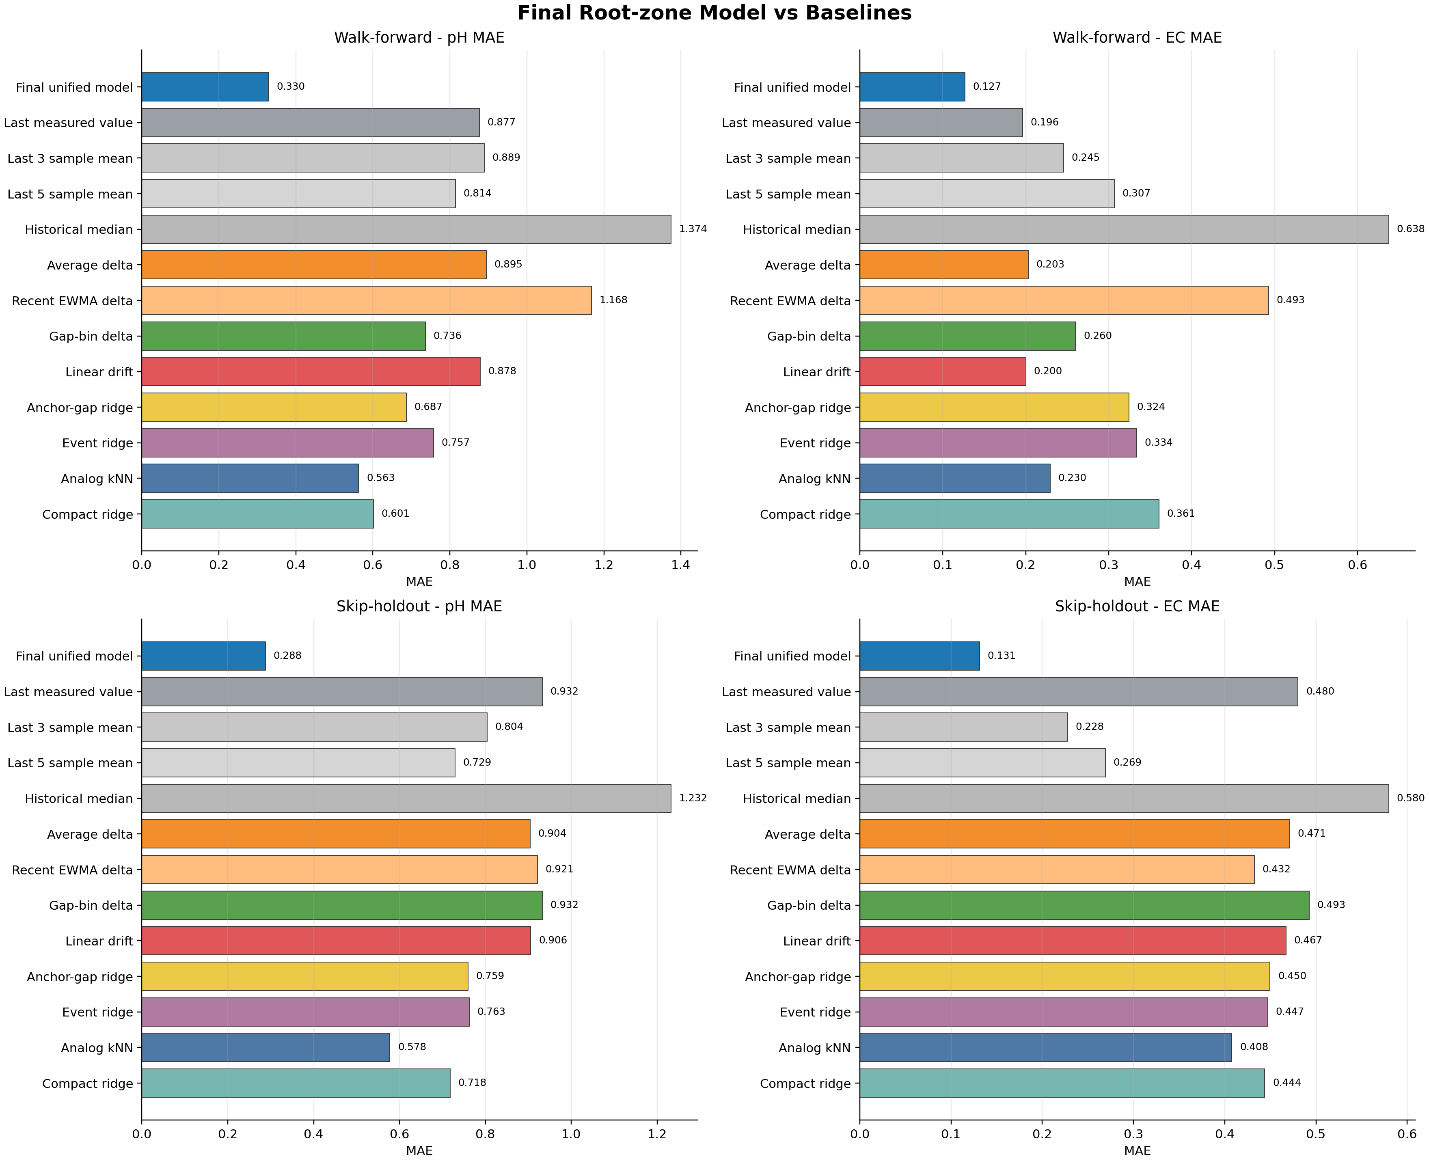
\includegraphics[width=\textwidth]{figures/fig12.png}
    \caption{\LR{Baseline Comparison -- Model vs.\ Naive Predictors}}
    \label{fig:baseline}
\end{figure}

איור \ref{fig:baseline} משווה את ביצועי המודל המאוחד הסופי מול מגוון בסיסי השוואה נאיביים (כגון שמירת הערך האחרון, ממוצע נע, וחיזוי מגמה ליניארית). בכל התרחישים -- הן ב-pH והן ב-EC, והן במבחן Walk-Forward והן במבחן Holdout -- המודל המאוחד מציג את שגיאת ה-MAE הנמוכה ביותר מבין כלל השיטות שנבחנו.

\subsection{אתגרים ודרכי פתרון}
במהלך הפיתוח נתקלנו בשישה אתגרים מרכזיים הנובעים מאופי הנתונים והמערכת. להלן הניתוח והפתרונות:

\subsubsection{"הקופסה השחורה" -- העדר ניטור רציף}
האתגר המרכזי בפרויקט הוא שבחממה הנחקרת לא הייתה מדידה רציפה של ערכי pH ו-EC בבית השורשים. ערכי האמת התקבלו מדגימות ידניות בלבד, ולכן רוב הזמן לא הייתה תמונת מצב ישירה של המצע. בין שתי דגימות ייתכנו שינויים משמעותיים במליחות או בחומציות, למשל בעקבות השקיה, דישון, אירוע חומצה, שטיפה או שינוי אקלימי, אך שינויים אלו אינם נמדדים באופן ישיר.

מצב זה יוצר "קופסה שחורה" תפעולית: ידועים לנו הקלטים למערכת, כגון מים, דשן, חומצה ותנאי סביבה, וידועות לנו נקודות מדידה בודדות של התוצאה, אך אין תיעוד רציף של התהליך שהתרחש ביניהן.

הפתרון שנבחר הוא פיתוח \SoftSensor{}, כלומר חיישן תוכנה. המודל אינו מתבסס על משוב רציף מחיישן קרקע, אלא לומד להעריך את מצב בית השורשים מתוך הנתונים הזמינים: מדידה ידועה אחרונה, תנאי אקלים ומיקרו-אקלים, השקיה, דישון, מצב הצמח והזמן שעבר עד נקודת החיזוי. בכך המודל מנסה לשחזר את הדינמיקה של המצע בין המדידות הישירות.

\subsubsection{בעיית הדלילות}
למרות שמסד הנתונים כולל אלפי רשומות אקלים ותפעול ברזולוציה של 10 דקות, מדידות היעד של pH ו-EC היו דלילות מאוד וכללו 109 נקודות מדידה בלבד. כלומר, קיימת אי-התאמה משמעותית בין כמות נתוני הקלט הצפופים לבין כמות ערכי האמת הזמינים לאימון המודל.

דלילות זו מעלה סיכון להתאמת יתר, משום שמודל מורכב עלול ללמוד רעש או תבניות מקריות במקום דפוסים כלליים. בנוסף, הדלילות מקשה על הערכת ביצועי המודל, מכיוון שכל נקודת מדידה משפיעה באופן משמעותי על המדדים הסופיים.

כדי להתמודד עם הבעיה, המודל נבנה על בסיס מרווחים בין נקודת בסיס $t_0$ לנקודת יעד $t_1$, ולא כחיזוי רציף של כל נקודת זמן. עבור כל מרווח חושבו משתני צבירה והיסטוריה המתארים את מה שהתרחש בין שתי המדידות. בנוסף, נעשה שימוש ב־\WFV{} ובבדיקת Holdout כדי לבחון את המודל בתרחיש שמדמה שימוש עתידי ולא חלוקה אקראית רגילה.

\subsubsection{רגישות המודל בערכי קיצון נמוכים}
חיזוי EC התגלה כמאתגר במיוחד בטווחי מוליכות נמוכים. בחלק ניכר מתקופת הניסוי נמדדו ערכי EC נמוכים יחסית, לעיתים סביב 0.2--0.5 mS/cm. בטווח כזה, שגיאה אבסולוטית קטנה עשויה להפוך לשגיאה יחסית גבוהה מאוד. לדוגמה, סטייה של 0.1 mS/cm היא קטנה מבחינה אבסולוטית, אך כאשר הערך האמיתי הוא 0.2 mS/cm היא מייצגת שגיאה יחסית של 50\%.

בעיה זו יוצרת קושי כפול. מצד אחד, מדדי שגיאה יחסית עלולים להחמיר יתר על המידה את הערכת המודל. מצד שני, כאשר הערכים נמוכים מאוד, יחס האות לרעש קטן: טעויות מדידה קטנות, השפעת טמפרטורה או שונות מקומית במצע עשויות להיות באותו סדר גודל כמו השינוי האמיתי בריכוז המלחים.

המשמעות האגרונומית היא שלא כל שגיאה יחסית גבוהה היא בהכרח משמעותית מבחינת קבלת החלטות. ההבדל בין EC של 0.2 ל-0.3 mS/cm עשוי להיות קטן מבחינה תפעולית, משום ששני הערכים עדיין מצביעים על מליחות נמוכה. לכן, בפרויקט הושם דגש על MAE, RMSE, \Rtwo{} והשוואה למודל נאיבי, ולא רק על אחוזי שגיאה.

כדי לשפר את יציבות החיזוי, ערכי EC עובדו באמצעות טרנספורמציה לוגריתמית של שינוי ה-EC. גישה זו מתאימה למשתני ריכוז, מפחיתה חיזויים לא פיזיקליים, ומסייעת למודל להתמודד טוב יותר עם טווחים נמוכים וגבוהים של מוליכות.

\subsubsection{אפקט הזיכרון ותלות במצב ההתחלתי}
בית השורשים אינו מגיב רק לפעולה האחרונה שבוצעה, אלא גם להיסטוריה הקודמת של המצע. לדוגמה, אותה מנת דשן עשויה לגרום לשינוי שונה לחלוטין אם היא ניתנת למצע שכבר רווי במלחים, לעומת מצע שטוף שבו ריכוז המלחים נמוך. באופן דומה, השקיה במים יכולה לגרום לדילול ולשטיפה, אך השפעתה תלויה במצב ההתחלתי, בנפח המים, בכמות הדשן ובזמן שעבר מאז אירועים קודמים.

בעיה זו מחייבת את המודל ללמוד תלות במצב. כלומר, לא מספיק לדעת מה קרה בין $t_0$ ל-$t_1$; יש צורך לדעת גם מאיזו נקודת פתיחה התחיל התהליך.

לכן הוכנסו למודל ערכי pH ו-EC בנקודת הבסיס, לצד משתני היסטוריה, משתני צבירה וחלונות זמן שונים. בנוסף, נבנו משתנים המייצגים יחסי ריכוז, כגון היחס בין כמות הדשן לבין נפח ההשקיה, כדי לייצג טוב יותר את אפקט המהילה ואת הריכוז בפועל של תמיסת ההזנה.

\subsubsection{אי-סדירות זמנית של הדגימות}
בניגוד לנתוני אקלים הנאספים כל 10 דקות, דגימות pH ו-EC לא נלקחו במרווחי זמן קבועים. לעיתים חלפו שעות בודדות בין שתי דגימות, ולעיתים יום או יותר. אי-סדירות זו מקשה על שימוש במודלים קלאסיים של סדרות עיתיות, המניחים לרוב צעד זמן קבוע.

המשמעות היא שהמודל אינו יכול להתייחס לכל מעבר בין דגימות כאילו הוא מייצג אותו פרק זמן. שינוי שהתרחש במשך שעתיים אינו שקול לשינוי שהתרחש במשך 48 שעות, גם אם בשני המקרים מדובר במעבר בין שתי מדידות עוקבות.

הפתרון היה להכניס למודל משתנה מפורש של משך הזמן בין $t_0$ ל-$t_1$, ולחשב את כלל משתני הצבירה ביחס לחלון הזמן הרלוונטי. כך המודל מקבל מידע גם על המצב ההתחלתי וגם על משך הזמן שבו הצטברו השפעות האקלים, ההשקיה והדישון.

\subsubsection{אי-רציפות בנתוני האקלים}
חלק ממדידות בית השורשים נאספו בתקופות שבהן לא היו זמינים נתוני מיקרו-אקלים פנימיים מלאים. מצב זה יצר בעיה משום שמודל בית השורשים זקוק למשתנים כגון טמפרטורה פנימית, לחות, קרינה, ET0 וטמפרטורת קרקע כדי לתאר את תנאי הסביבה שהשפיעו על הצמח והמצע.

ויתור על תקופות אלו היה מצמצם עוד יותר את מספר דגימות היעד, שגם כך היה מוגבל. לכן פותח מודל מיקרו-אקלים שלמד את הקשר בין נתוני התחנה החיצונית לבין התנאים בתוך החממה ובסביבת המצע.

באמצעות מודל זה ניתן היה להשלים או לחזות משתנים פנימיים חסרים, וליצור רצף נתונים מלא יותר עבור מודל בית השורשים. פתרון זה אפשר לנצל טוב יותר את מדידות ה-pH וה-EC הקיימות, ולשמור על עקביות בין שלב האקלים לבין שלב חיזוי בית השורשים.

\section{יישום המודל בממשק דיגיטלי תומך החלטה}
כחלק מהמעבר ממודל מחקרי לכלי יישומי, פותח ממשק דיגיטלי המאפשר להריץ את שרשרת החיזוי ללא צורך בכתיבת קוד. מטרת הממשק היא להנגיש את מודל החיזוי למשתמש תפעולי, ולאפשר קבלת תחזית עתידית של ערכי pH ו-EC בבית השורשים על בסיס נתוני אקלים, קרינה, השקיה, דישון ומדידה נוכחית ידועה.

הממשק משמש כשכבת הפעלה מעל המודלים שפותחו בפרויקט: תחילה מופעל מודל המיקרו-אקלים, אשר יוצר תחזית של תנאי הסביבה בתוך החממה, ולאחר מכן מופעל מודל בית השורשים, המשתמש בתחזית זו יחד עם נתוני הממשק החקלאי כדי לחזות את מצב ה-pH וה-EC בנקודת זמן עתידית.

\subsection{מטרת הממשק}
הממשק נועד לגשר בין שלב הפיתוח המחקרי לבין שימוש מעשי במודל. בעוד שבשלב המחקר המודלים הופעלו באמצעות מחברות Jupyter וקוד Python, הממשק מאפשר למשתמש להזין נתונים בצורה מובנית, להריץ את המודלים ולקבל פלט ברור של תחזית בית השורשים.

באופן זה, המערכת הופכת את מודל ה־\SoftSensor{} לכלי תומך החלטה ראשוני. המשתמש אינו נדרש להבין את פרטי המימוש של המודל, אלא רק לספק את הקלטים הדרושים: נתוני מזג אוויר וקרינה, ערכי pH ו-EC נוכחיים, מועד החיזוי, ונתוני אירועי השקיה ודישון רלוונטיים.

\subsection{מבנה תהליך העבודה בממשק}
תהליך העבודה בממשק מחולק לארבעה שלבים מרכזיים:

\begin{enumerate}
    \item \textbf{העלאת נתוני אקלים וקרינה:} בשלב הראשון המשתמש מעלה קובצי מזג אוויר וקרינה. המערכת תומכת בקבצים בפורמטים נפוצים כגון CSV, Excel ו-JSON. נתונים אלו משמשים כקלט למודל המיקרו-אקלים.
    \item \textbf{יצירת תחזית מיקרו-אקלים:} לאחר העלאת הקבצים, המערכת מפעילה את מודל המיקרו-אקלים ומייצרת תחזית של משתנים פנימיים בחממה, כגון טמפרטורה, לחות, ET0, קרינה פנימית וטמפרטורת קרקע. תחזית זו נשמרת כקובץ פלט, ומשמשת בהמשך כקלט למודל בית השורשים.
    \item \textbf{הזנת מצב בית השורשים ואירועים תפעוליים:} בשלב זה המשתמש מזין את נקודת הבסיס של החיזוי: זמן המדידה הנוכחית, ערכי pH ו-EC נוכחיים, זמן היעד לחיזוי, תאריך שתילה וכיסוי נוף. בנוסף, ניתן להזין אירועי השקיה, דישון, חומצה, Gypsum ו-Kortin שהתרחשו לפני ואחרי נקודת הבסיס. אירועים אלו מספקים למודל את ההקשר התפעולי הנדרש להבנת מצב המצע.
    \item \textbf{הרצת מודל בית השורשים וקבלת תחזית:} לאחר הזנת כל הקלטים, המערכת מפעילה את מודל בית השורשים ומחזירה תחזית לערכי pH ו-EC בנקודת הזמן העתידית. בנוסף, הממשק מציג את פער הזמן בין נקודת הבסיס לנקודת היעד, ומאפשר הורדת קובצי הפלט לצורך תיעוד או ניתוח נוסף.
\end{enumerate}

\begin{figure}[H]
    \centering
    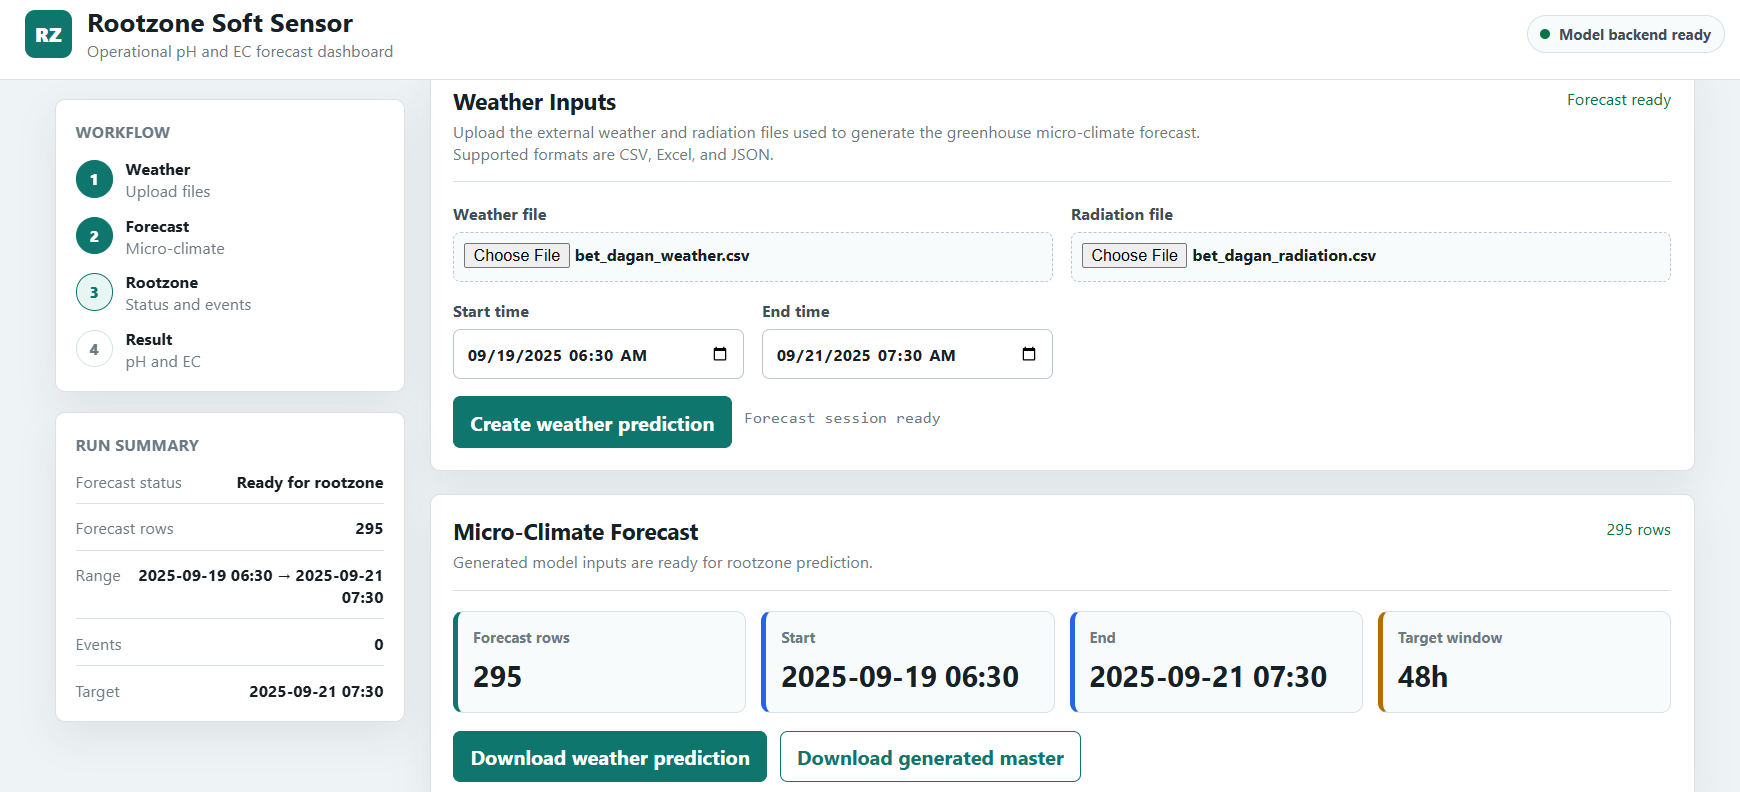
\includegraphics[width=0.95\textwidth]{figures/fig13.png}
    \caption{\LR{Digital Interface -- Weather Upload and Climate Forecast}}
    \label{fig:interface1}
\end{figure}

\begin{figure}[H]
    \centering
    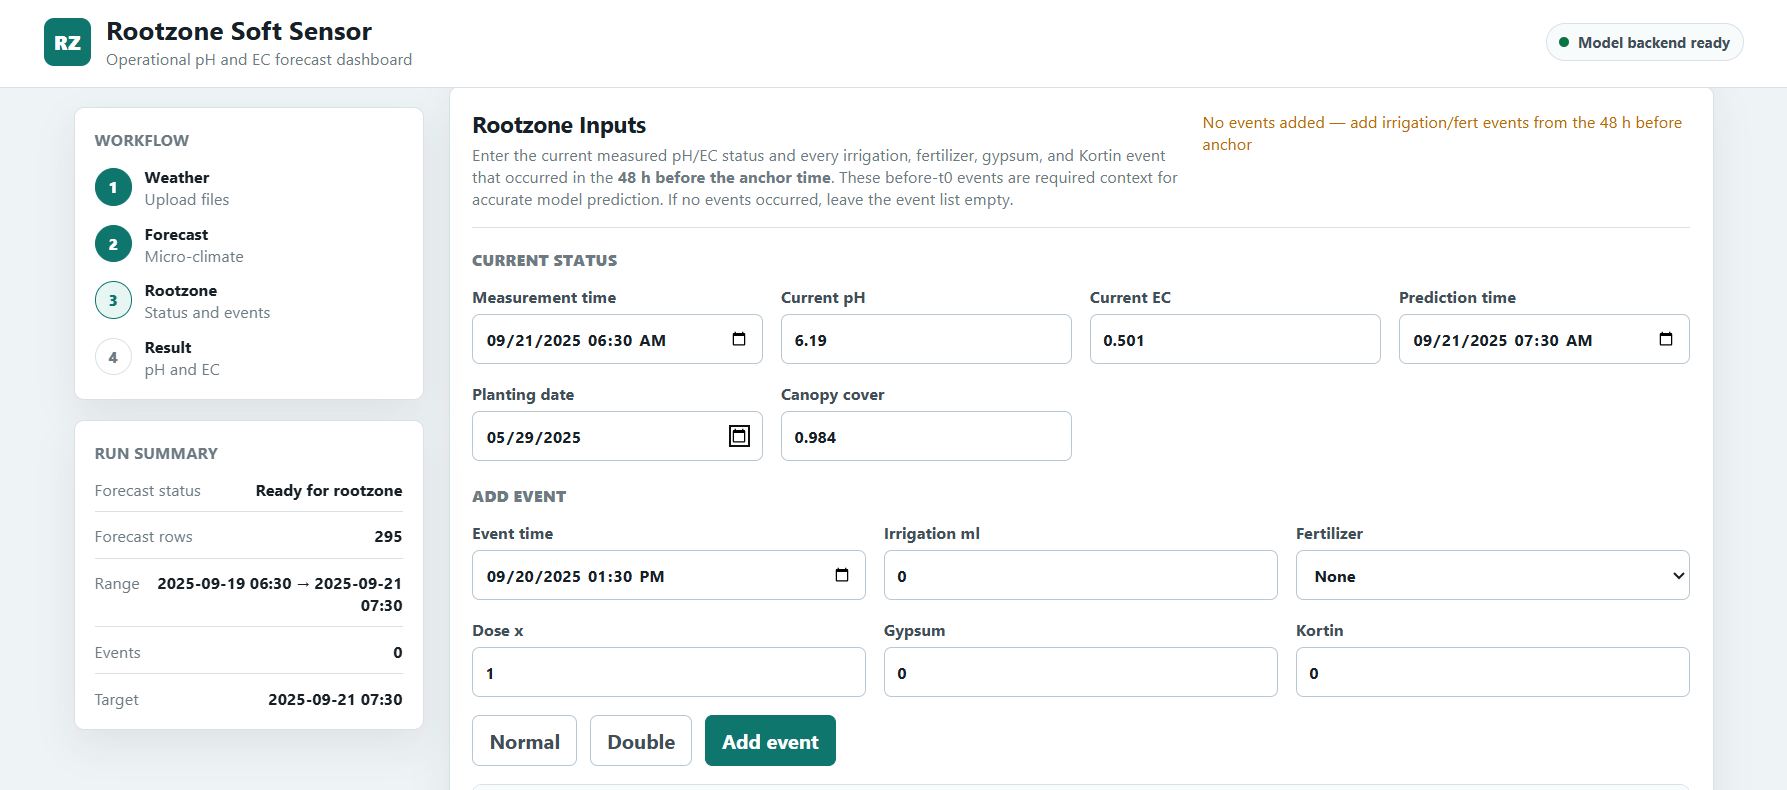
\includegraphics[width=0.95\textwidth]{figures/fig14.png}
    \caption{\LR{Digital Interface -- Operational Inputs}}
    \label{fig:interface2}
\end{figure}

\begin{figure}[H]
    \centering
    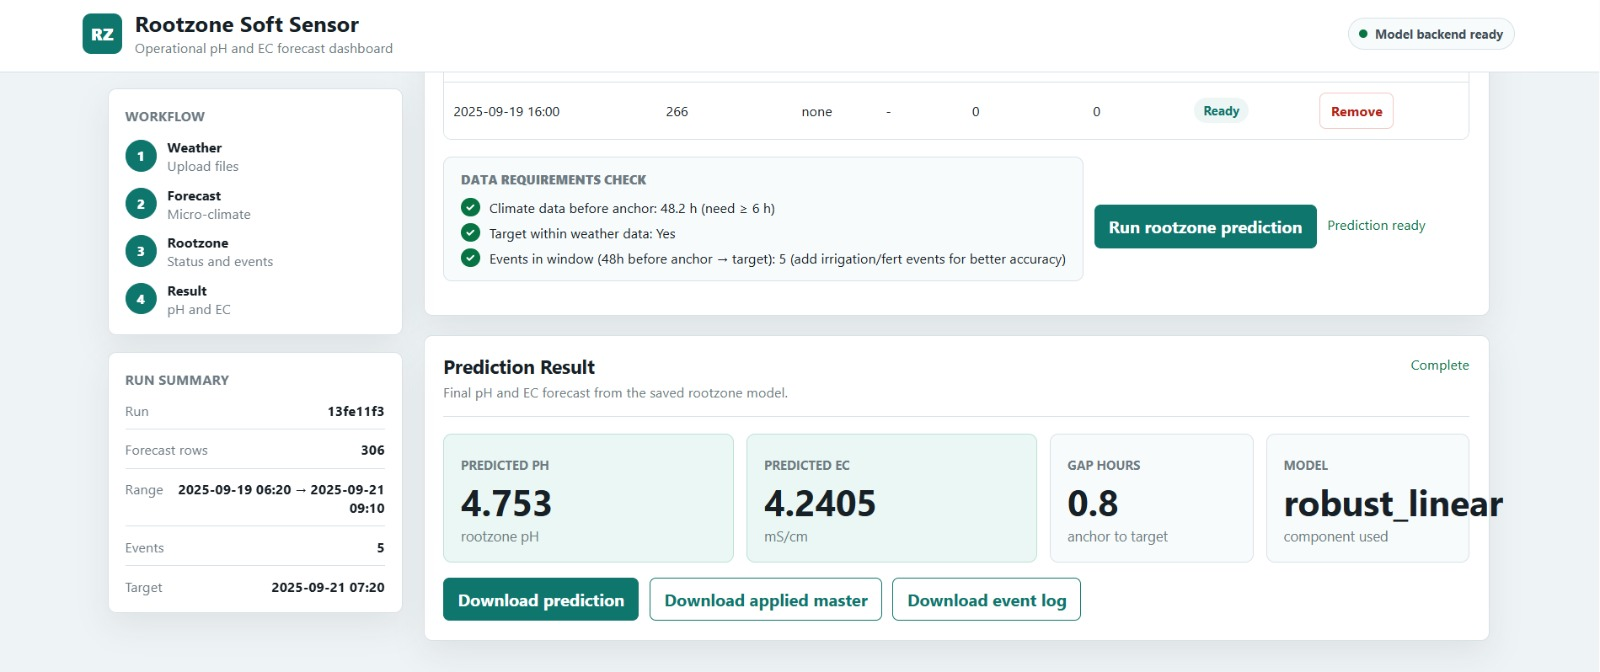
\includegraphics[width=0.95\textwidth]{figures/fig15.jpeg}
    \caption{\LR{Digital Interface -- Rootzone pH and EC Forecast}}
    \label{fig:interface3}
\end{figure}

\subsection{קלטי ופלטי המערכת}
הממשק מקבל מספר קבוצות קלט מרכזיות. תחילה מוזנים קובצי מזג אוויר וקרינה, המשמשים ליצירת תחזית מיקרו-אקלים בתוך החממה. לאחר מכן מוזנים ערכי pH ו-EC נוכחיים, זמן המדידה, זמן היעד לחיזוי, נתוני מצב הצמח, ואירועי השקיה ודישון שהתרחשו בפרק הזמן הרלוונטי.

שילוב קלטים אלו מאפשר למודל להתייחס לא רק למצב הנוכחי של בית השורשים, אלא גם לתנאים הסביבתיים ולפעולות הממשק שהתרחשו בין נקודת הבסיס לנקודת החיזוי. בכך הממשק משמר את מבנה החיזוי של המודל, המבוסס על מעבר מ-$t_0$ ל-$t_1$ ולא על חיזוי רגעי מנותק מהקשר.

פלטי המערכת כוללים את ערך ה-pH החזוי, ערך ה-EC החזוי ביחידות mS/cm, מספר השעות בין נקודת הבסיס לנקודת היעד, וקובצי פלט להורדה. קבצים אלו כוללים את תחזית המיקרו-אקלים, טבלת הנתונים המעובדת ותחזית בית השורשים, ויכולים לשמש לתיעוד, בדיקה או ניתוח נוסף.

\subsection{חשיבות הממשק בפרויקט}
הממשק הדיגיטלי מהווה שלב חשוב בהפיכת המודל מכלי מחקרי לכלי תומך החלטה יישומי. הוא מאפשר להפעיל את שרשרת החיזוי בצורה מובנית, להפחית תלות בקוד, ולבדוק כיצד המודל עשוי להשתלב בתהליך עבודה חקלאי.

עם זאת, בשלב הנוכחי הממשק אינו מהווה מערכת בקרה אוטונומית ואינו מחליף שיקול דעת מקצועי או מדידות ידניות. תפקידו הוא לספק הערכה עתידית של מצב בית השורשים, שתוכל לסייע למגדל או לאגרונום לזהות מגמות אפשריות ולקבל החלטות מושכלות יותר לגבי השקיה, דישון או צורך במדידה נוספת.

\section{דיון}
תוצאות הפרויקט מצביעות על כך שניתן לפתח מודל חיזוי מבוסס נתונים להערכת משתני בית השורשים בחממה, גם כאשר מדידות היעד של pH ו-EC דלילות יחסית. שילוב נתוני אקלים, מיקרו-אקלים, השקיה, דישון, מצב הצמח ומדידות עבר אפשר למודל ללמוד את הדינמיקה הכללית של המצע ולספק תחזית עתידית בעלת ערך תפעולי.

\subsection{משמעות תוצאות מודל המיקרו-אקלים}
מודל המיקרו-אקלים הציג ביצועים טובים בחיזוי המשתנים המרכזיים בתוך החממה, ובהם טמפרטורת אוויר פנימית, לחות יחסית, קרינה פנימית, ET0 וטמפרטורת קרקע. תוצאות אלו חשובות משום שבית השורשים אינו מושפע ישירות רק מנתוני התחנה המטאורולוגית החיצונית, אלא מהתנאים בפועל בתוך סביבת הגידול.

הדיוק הגבוה של מודל המיקרו-אקלים מאפשר להשתמש בו כשכבת קלט יציבה עבור מודל בית השורשים. במילים אחרות, המודל יוצר בסיס סביבתי רציף שמאפשר לחזות את תגובת המצע גם כאשר אין מדידה ישירה מלאה של כל משתני החממה בכל רגע.

\subsection{משמעות תוצאות מודל בית השורשים}
מודל בית השורשים הצליח לחזות את ערכי pH ו-EC ברמת דיוק טובה ביחס למודל נאיבי המבוסס על שמירת הערך האחרון שנמדד. עבור pH התקבלה יציבות גבוהה יחסית הן במבחן Walk-Forward והן במבחן Holdout, דבר המצביע על כך שהמודל מצליח ללמוד את דפוסי השינוי המרכזיים של החומציות במצע.

עבור EC התקבלו גם כן ביצועים טובים מבחינת MAE ו-\Rtwo{}, אך החיזוי נותר מורכב יותר. הסיבה המרכזית לכך היא שערכי EC נמוכים גורמים לכך שגם סטייה אבסולוטית קטנה מתורגמת לשגיאה יחסית גבוהה. לכן, בהערכת ביצועי EC חשוב להתייחס לא רק לאחוזי השגיאה, אלא גם למשמעות האגרונומית של הסטייה.

\subsection{תרומת הגישה ההיברידית}
אחד היתרונות המרכזיים של המודל הוא השילוב בין רכיב \GB{} לבין רכיב ליניארי חסין. רכיב ה־\GB{} מאפשר ללמוד קשרים מורכבים ולא-ליניאריים מתוך דפוסים שנצפו בנתוני העבר, ואילו הרכיב הליניארי מסייע בהתמודדות עם מגמות ואירועים תפעוליים בעלי השפעה גבוהה.

שילוב זה מאפשר למודל לבצע אינטרפולציה בתוך תחומי התנהגות מוכרים, ובמקביל לבצע אקסטרפולציה זהירה במצבים שבהם מופיעים אירועים פחות שכיחים. בכך המודל מתאים יותר למערכת חקלאית דינמית, שבה קיימים גם דפוסים מחזוריים וגם אירועים נקודתיים חריגים.

\subsection{מגבלות המחקר}
למרות התוצאות החיוביות, קיימות מספר מגבלות שיש לקחת בחשבון. ראשית, מספר מדידות היעד של pH ו-EC היה מוגבל יחסית, ולכן יש צורך בהמשך איסוף נתונים כדי לשפר את הכללת המודל. שנית, המודל נבחן על בסיס עונת גידול אחת, ולכן עדיין לא ניתן לקבוע בוודאות את ביצועיו בעונות אחרות, בגידולים אחרים או בחממות שונות.

בנוסף, בדיקת ה-Holdout בוצעה מתוך אותה עונת גידול, ולכן היא אינה מחליפה בדיקה מלאה על עונת גידול עתידית עצמאית. כמו כן, המדידות הידניות עצמן עשויות לכלול רעש, שונות מרחבית או טעויות מדידה, ולכן חלק מהשגיאה של המודל עשוי לנבוע גם מאי-ודאות במדידת היעד.

\subsection{משמעות יישומית}
המשמעות היישומית של הפרויקט היא שניתן להשתמש במודל כ־\SoftSensor{} תומך החלטה לניהול בית השורשים. המודל אינו מחליף מדידות ידניות או שיקול דעת אגרונומי, אך הוא יכול לסייע בהערכת המגמה בין מועדי המדידה, בזיהוי מוקדם של סיכון לשינויי pH או EC, ובתכנון מושכל יותר של השקיה ודישון.

בכך הפרויקט מדגים מעבר מגישה תגובתית, שבה מתקנים חריגות לאחר שהן נמדדו, לגישה פרואקטיבית יותר, שבה ניתן להעריך מראש את כיוון השינוי הצפוי ולתמוך בקבלת החלטות בזמן.

\section{מסקנות}
בפרויקט זה פותחה מערכת חיזוי מבוססת למידת מכונה להערכת משתני בית השורשים בחממה, תוך שילוב נתוני אקלים, מיקרו-אקלים, השקיה, דישון, מצב הצמח ומדידות עבר של pH ו-EC.

המסקנות המרכזיות הן:

\begin{itemize}
    \item ניתן לבנות מסד נתונים מאוחד המשלב מקורות מידע הטרוגניים ברזולוציות זמן שונות, ולהפוך אותם לבסיס מתאים לאימון מודל חיזוי.
    \item מודל המיקרו-אקלים מספק תחזית אמינה של תנאי הסביבה בתוך החממה, ומשמש שכבת קלט חשובה למודל בית השורשים.
    \item מודל בית השורשים מצליח לחזות את ערכי pH ו-EC בדיוק טוב, ומשפר את הביצועים ביחס למודל נאיבי המבוסס על שמירת הערך האחרון שנמדד.
    \item חיזוי pH התגלה כיציב יחסית, בעוד שחיזוי EC מאתגר יותר בעיקר בטווחי מוליכות נמוכים.
    \item הגישה ההיברידית, המשלבת \GB{} עם רכיב ליניארי חסין, מאפשרת להתמודד טוב יותר עם שילוב של דפוסים מוכרים ואירועים תפעוליים בעלי השפעה גבוהה.
    \item הממשק הדיגיטלי שפותח מדגים כיצד ניתן להנגיש את המודל למשתמש תפעולי ולהפוך אותו לכלי תומך החלטה ראשוני.
\end{itemize}

בסיכום, הפרויקט מדגים היתכנות לפיתוח \SoftSensor{} לחיזוי pH ו-EC בבית השורשים, ומראה כי למידת מכונה יכולה לתרום לניהול מדויק ופרואקטיבי יותר של השקיה ודישון בחממות.

\section{ביבליוגרפיה}

\newcommand{\refentry}[1]{\par\noindent #1\par\smallskip}

\begingroup
\setmainlanguage{english}
\setlength{\parindent}{0pt}
\begin{LTR}

\refentry{Moon, T., Ahn, T. I., \& Son, J. E. (2018). Forecasting Root-Zone Electrical Conductivity of Nutrient Solutions in Closed-Loop Soilless Cultures via a Recurrent Neural Network Using Environmental and Cultivation Information. \textit{Frontiers in Plant Science}, 9, 859.}

\refentry{Lü, X., Nurmemet, I., Xiao, S., Zhao, J., Yu, X., Aili, Y., \& Li, S. (2025). Spatial-temporal simulation and prediction of root zone soil moisture based on Hydrus-1D and CNN-LSTM-attention models in Yutian Oasis, southern Xinjiang, China. \textit{Pedosphere}, 35(5), 846--857.}

\refentry{Cai, Y., Zheng, Y., \& Zhang, Y. (2023). Extrapolated Random Tree for Regression. \textit{Proceedings of the 40th International Conference on Machine Learning (ICML)}, PMLR 202.}

\refentry{Friedberg, R., Tibshirani, J., Athey, S., \& Wager, S. (2021). Local linear forests. \textit{Journal of Computational and Graphical Statistics}, 30(2), 503--517.}

\refentry{Loh, W. Y., Wei, Z., \& Formann, A. (2007). Extrapolation errors in linear model trees. \textit{ACM Transactions on Knowledge Discovery from Data (TKDD)}, 1(2), 6-es.}

\refentry{Muckley, E. S., Saal, J. E., Meredig, B., et al. (2023). Interpretable models for extrapolation in scientific machine learning. \textit{Digital Discovery}, 2(3), 643--653.}

\end{LTR}
\endgroup


\end{document}
%========== End of the document ==========
